% !TeX spellcheck = pt_BR
\documentclass[12pt,portuguese]{article}

%----------------------------------------------------------------------
% PACOTES ESSENCIAIS E TRADUÇÃO
%----------------------------------------------------------------------
\usepackage[brazilian]{babel}     % Suporte à língua portuguesa
\usepackage[utf8]{inputenc}       % Codificação de entrada
\usepackage[T1]{fontenc}          % Codificação da fonte
\usepackage{lmodern}              % Fonte escalável
\usepackage{microtype}            % Microtipografia (expansão e protrusão)

%----------------------------------------------------------------------
% PACOTES MATEMÁTICOS
%----------------------------------------------------------------------
\usepackage{amsmath, amsthm, amssymb, amstext, mathtools}
\usepackage{mathrsfs}             % Para fontes como \mathscr
\usepackage{dsfont}               % Para o indicador de conjunto \mathds{1}
\usepackage[all]{xy}              % Para diagramas comutativos
\usepackage{imakeidx}             % Criação de Lista de Símbolos / Índice

% Desigualdades sempre com símbolos inclinados
\let\leq\leqslant
\let\le\leqslant
\let\ge\geqslant
\let\geq\geqslant

%----------------------------------------------------------------------
% FORMATAÇÃO, LAYOUT E CORES
%----------------------------------------------------------------------
\usepackage{geometry}
\usepackage{varwidth}
\usepackage{graphicx}
\usepackage[pdftex]{xcolor}
\usepackage{titlesec}
\usepackage{appendix}
\usepackage{enumitem}
\usepackage{float}
\usepackage{booktabs}
\usepackage{array}
\usepackage{colortbl}
\usepackage{fontawesome5}
\usepackage{lucide-icons}
\usepackage{caption}
\usepackage{stackengine}
\captionsetup{width=0.8\textwidth}

% Definição de Cores
\definecolor{teal}{RGB}{15,118,110}
\definecolor{text}{RGB}{28,25,23}
\definecolor{muted}{RGB}{87,83,78}
\definecolor{card}{RGB}{255,255,255}
\definecolor{border}{RGB}{231,229,228}

% Definição de margens e espaçamento
\setlength{\topmargin}{-0.7in}
\setlength{\oddsidemargin}{0in}
\setlength{\textheight}{9.55in}
\setlength{\textwidth}{6.5in}
\setlength{\baselineskip}{12mm}

% Formatação dos títulos de seção
\titleformat{\section}{\Large\bfseries}{\thesection.}{0.5em}{}
\titleformat{\subsection}{\large\bfseries}{\thesubsection.}{0.5em}{}
\titleformat{\subsubsection}{\normalfont\itshape}{\thesubsubsection.}{0.6em}{}

%----------------------------------------------------------------------
% TIKZ E GRÁFICOS
%----------------------------------------------------------------------
\usepackage{tikz}
\usepackage{pgfplots}
\pgfplotsset{compat=1.17}
\usetikzlibrary{positioning,calc,fit,backgrounds,nfold,decorations.pathreplacing,calligraphy,tikzmark,patterns,arrows.meta,bending,hobby}

%----------------------------------------------------------------------
% REFERÊNCIAS, LINKS E METADADOS DO PDF
%----------------------------------------------------------------------
\usepackage[pdftex, colorlinks, linkcolor={red!50!black}, 
citecolor={red}, urlcolor={blue!80!black}]{hyperref}

\hypersetup{
pdftitle={Passeios Aleatórios},
pdfauthor={L. Cioletti},
pdfsubject={processos estocásticos, passeios aleatórios, probabilidades de transição, recorrência, transiência, problema da ruína do jogador},
pdfkeywords={passeios aleatórios, processos estocásticos, recorrência, transiência, ruína do jogador, MAT-UnB}
}

% --- PACOTE E COMANDO PARA A LICENÇA CREATIVE COMMONS ---
\usepackage[type={CC},modifier={by-nc-sa},version={4.0}]{doclicense}
\newcommand\blfootnote[1]{%
\begingroup
\renewcommand\thefootnote{}\footnote{#1}%
\addtocounter{footnote}{-1}%
\endgroup
}

%----------------------------------------------------------------------
% ALIASCNT E AMBIENTES DE TEOREMA (Cleveref)
%----------------------------------------------------------------------
\usepackage{aliascnt}
\theoremstyle{definition}
\newtheorem{theorem}{Teorema}

\newaliascnt{definition}{theorem}
\newtheorem{definition}[definition]{Definição}
\aliascntresetthe{definition}

\newaliascnt{example}{theorem}
\newtheorem{example}[example]{Exemplo}
\aliascntresetthe{example}

\newaliascnt{proposition}{theorem}
\newtheorem{proposition}[proposition]{Proposição}
\aliascntresetthe{proposition}

\newaliascnt{corollary}{theorem}
\newtheorem{corollary}[corollary]{Corolário}
\aliascntresetthe{corollary}

\newaliascnt{lemma}{theorem}
\newtheorem{lemma}[lemma]{Lema}
\aliascntresetthe{lemma}

\newaliascnt{remark}{theorem}
\newtheorem{remark}[remark]{Observação}
\aliascntresetthe{remark}

% O primeiro argumento é o espaço acima do ambiente. Acrescentamos 0,4 cm ao
% valor usual de 3pt para separar melhor os exercícios.
\newtheoremstyle{plainexercise}
  {14.4pt}{3pt}{\normalfont}{}{\bfseries}{.}{.5em}
  {\thmnumber{#2}\thmnote{ #3}}
\theoremstyle{plainexercise}
\newtheorem{exercise}{Exercício}

% Versão marcada dos exercícios: a estrela fica pendurada na margem esquerda,
% como nas notas anteriores.
\newtheoremstyle{starredexercise}
  {14.4pt}{3pt}{\normalfont}{}{\bfseries}{.}{.5em}
  {\llap{\textasteriskcentered\,}\thmnumber{#2}\thmnote{ #3}}
\theoremstyle{starredexercise}
\newtheorem{starredexercise}[exercise]{Exercício}
\theoremstyle{definition}

% Ambientes não numerados usados no texto
\newtheorem*{property}{Propriedade}
\newtheorem*{solution}{Solução}

% Se um enumerate for o primeiro conteúdo de um teorema/exercício (cabeçalho
% ainda pendente, \@inlabel true), o \leavevmode dispara o \everypar do amsthm
% que coloca o cabeçalho na própria linha, antes da lista iniciar.
\makeatletter
\setlist[enumerate]{before={\if@inlabel\leavevmode\fi}}
\makeatother

% Nomes em português para os ambientes
\AtBeginDocument{\renewcommand{\proofname}{\normalfont\textbf{Prova}}}
\renewcommand{\qedsymbol}{$\blacksquare$}

% Cleveref (deve vir depois de hyperref e amsthm)
\usepackage[brazilian,nameinlink]{cleveref}

\crefname{theorem}{teorema}{teoremas}
\Crefname{theorem}{Teorema}{Teoremas}
\crefname{definition}{definição}{definições}
\Crefname{definition}{Definição}{Definições}
\crefname{lemma}{lema}{lemas}
\Crefname{lemma}{Lema}{Lemas}
\crefname{proposition}{proposição}{proposições}
\Crefname{proposition}{Proposição}{Proposições}
\crefname{corollary}{corolário}{corolários}
\Crefname{corollary}{Corolário}{Corolários}
\crefname{example}{exemplo}{exemplos}
\Crefname{example}{Exemplo}{Exemplos}
\crefname{exercise}{exercício}{exercícios}
\Crefname{exercise}{Exercício}{Exercícios}
\crefname{remark}{observação}{observações}
\Crefname{remark}{Observação}{Observações}
\crefname{section}{seção}{seções}
\Crefname{section}{Seção}{Seções}

%----------------------------------------------------------------------
% MACROS ADICIONAIS
%----------------------------------------------------------------------
\let\oldemptyset\emptyset
\let\emptyset\varnothing
\graphicspath{{./}{../arquivos-aux/}}

% Seno na convenção em português
\renewcommand{\sin}{\operatorname{sen}}

% Evita hifenização e quebra de sílabas no abstract mantendo a justificação
\expandafter\def\expandafter\abstract\expandafter{%
  \abstract
  \hyphenpenalty=10000
  \exhyphenpenalty=10000
  \emergencystretch=1.5em
}

%----------------------------------------------------------------------
% DOCUMENTO PRINCIPAL
%----------------------------------------------------------------------
\begin{document}

% --- CABEÇALHO COM O LOGO DA UnB ---
\vspace*{-0.8cm}
\begin{figure}[H]

\includegraphics{logo-mat-unb.pdf}
\end{figure}

% --- TÍTULO, AUTOR E DATA ---
\vspace*{0.3cm}
\begin{center}
{\LARGE\bf Passeios Aleatórios}
\vspace{1cm}

{\large \bf L. Cioletti}
\vspace{0.3cm}

{\footnotesize Novembro de 2026}
\end{center}

% --- LICENÇA NO RODAPÉ ---
\blfootnote{%
\doclicenseImage[imagewidth=2.6em]\
\begingroup
\hypersetup{urlcolor=darkgray}
\href{\doclicenseURL}{%
\doclicenseName{} -- Attribution-NonCommercial-ShareAlike 4.0 International%
}%
\endgroup
}

% --- RESUMO (ABSTRACT) ---
\begin{abstract}
Nestas notas de aula, iniciamos o estudo dos passeios aleatórios, uma das
classes mais simples e versáteis de processos estocásticos a tempo discreto.
Começamos com a formulação rigorosa do passeio aleatório simples
unidimensional nos inteiros, distinguindo o caso simétrico do caso
assimétrico, e apresentamos um modelo de apostas como motivação inicial.
Em seguida, calculamos as probabilidades de transição e de retorno à origem,
investigamos o comportamento assintótico dessas probabilidades com o auxílio
da Fórmula de Stirling e demonstramos o critério que separa a recorrência da
transiência em uma dimensão. Por fim, resolvemos o clássico Problema da Ruína
do Jogador tanto no cenário com duas barreiras finitas quanto no caso de um
adversário infinitamente rico, determinando ainda o número médio de jogadas
até o término do jogo. O texto inclui figuras ilustrativas, exemplos
detalhados e uma lista de exercícios e problemas. A exposição é baseada no
Capítulo~10 da referência \cite{GrimmettWelsh2014}.
\end{abstract}

\section{Passeios Aleatórios Unidimensionais}\label{sec:passeios-unidimensionais}

Nas notas de aula anteriores sobre processos de ramificação, iniciamos o
estudo de fenômenos que evoluem aleatoriamente ao longo do tempo. Nestas
notas, damos sequência a esse programa examinando uma segunda classe
fundamental de processos estocásticos: os passeios aleatórios.

Há muitos exemplos práticos de passeios aleatórios. Diversos processos na
física envolvem partículas atômicas e subatômicas que migram pelo espaço que
habitam, e frequentemente podemos modelar esses deslocamentos por meio de
passeios aleatórios. Além disso, passeios aleatórios surgem em contextos não
físicos, como em modelos de jogos de azar, propagação de epidemias e
oscilações de índices do mercado financeiro. Estudaremos aqui apenas o tipo
mais simples de passeio aleatório, formulado em termos de uma partícula
hipotética que se move aleatoriamente sobre um conjunto unidimensional, isto
é, sobre uma reta, à medida que o tempo avança.

Para simplificar, supomos que tanto o espaço quanto o tempo são
\emph{discretos}. Observamos a posição da partícula nos instantes discretos
$0, 1, 2, \ldots$ e assumimos que, em cada um desses instantes, ela ocupa uma
das posições inteiras $\ldots, -2, -1, 0, 1, 2, \ldots$ da reta real. A
dinâmica do movimento é descrita da seguinte maneira. Seja $p$ um número real
satisfazendo $0 < p < 1$, e defina $q = 1 - p$. A cada unidade de tempo, a
partícula desloca-se uma unidade para a esquerda, com probabilidade $q$, ou
uma unidade para a direita, com probabilidade $p$. Mais precisamente, se $S_n$
denota a posição da partícula no instante $n$, então
\[
  S_{n+1} =
  \begin{cases}
    S_n + 1, & \text{com probabilidade } p, \\
    S_n - 1, & \text{com probabilidade } q,
  \end{cases}
\]
e supomos que a direção aleatória de cada salto é independente de todos os
saltos anteriores.

Para formalizar essa construção em termos de variáveis aleatórias, convém
escrever cada posição como a soma acumulada dos deslocamentos individuais.
Assim, temos
\begin{equation}\label{eq:passeio-soma}
  S_n = S_0 + X_1 + X_2 + \cdots + X_n \qquad \text{para } n = 0, 1, 2, \ldots,
\end{equation}
com $S_0$ sendo a posição inicial (com a convenção de que a soma vazia vale
zero quando $n = 0$) e com $(X_n)_{n \geqslant 1}$ uma sequência de variáveis
aleatórias independentes e identicamente distribuídas, cada uma com
distribuição
\begin{align*}
\mathbb{P}(X_j=-1)= q \qquad \text{e}\qquad \mathbb{P}(X_j=1)=p,
\end{align*}
onde $p+q=1$. Chamamos o processo $(S_n)_{n \geqslant 0}$ de \emph{passeio aleatório simples}. Dizemos
que o passeio é \emph{simétrico} se $p = q = \tfrac{1}{2}$, e
\emph{assimétrico} caso contrário.

A \Cref{fig:trajetorias-passeio-1d} ilustra trajetórias típicas desses dois
tipos de passeios começando na origem $S_0 = 0$. No caso simétrico, o passeio oscila sem
direção preferencial em torno do ponto de partida. 
Por outro lado, no caso assimétrico com
$p > \tfrac{1}{2}$, o deslocamento médio de $2p - 1$ por passo tende a afastar
a partícula para a direita à medida que $n$ cresce.

\begin{figure}[htbp]
  \centering
  \begin{tikzpicture}[
    x=0.48cm, y=0.45cm,
    >=Stealth,
    font=\small,
  ]
    % Painel esquerdo: passeio simétrico (p = 1/2)
    \begin{scope}
      % Grade leve
      \foreach \y in {-2, 2, 4, 6} {
        \draw[black!16, densely dashed, line width=0.4pt] (0, \y) -- (12, \y);
      }

      % Eixos
      \draw[->, black!65, line width=0.55pt] (-0.4, 0) -- (12.8, 0)
        node[right=2pt, font=\small, text=text] {$n$};
      \draw[->, black!65, line width=0.55pt] (0, -3.4) -- (0, 7.4)
        node[above=2pt, font=\small, text=text] {$S_n$};

      % Ticks nos eixos
      \foreach \x in {2, 4, 6, 8, 10, 12} {
        \draw[black!55, line width=0.45pt] (\x, -0.15) -- (\x, 0.15);
        \node[below=2pt, font=\scriptsize, text=muted, fill=white, inner sep=1pt]
          at (\x, -0.15) {$\x$};
      }
      \foreach \y in {-2, 2, 4, 6} {
        \draw[black!55, line width=0.45pt] (-0.15, \y) -- (0.15, \y);
        \node[left=2pt, font=\scriptsize, text=muted] at (-0.15, \y) {$\y$};
      }
      \node[below left=2pt, font=\scriptsize, text=muted] at (0, 0) {$0$};

      % Trajetória simétrica: 0, 1, 0, -1, -2, -1, 0, 1, 2, 1, 0, -1, 0
      \draw[teal, line width=1.35pt]
        (0,0) -- (1,1) -- (2,0) -- (3,-1) -- (4,-2) -- (5,-1) -- (6,0)
        -- (7,1) -- (8,2) -- (9,1) -- (10,0) -- (11,-1) -- (12,0);
      \foreach \x/\y in {
        0/0, 1/1, 2/0, 3/-1, 4/-2, 5/-1, 6/0,
        7/1, 8/2, 9/1, 10/0, 11/-1, 12/0
      } {
        \fill[teal] (\x, \y) circle (1.6pt);
      }
    \end{scope}

    % Painel direito: passeio assimétrico (p = 3/4)
    \begin{scope}[xshift=7.8cm]
      % Grade leve
      \foreach \y in {-2, 2, 4, 6} {
        \draw[black!16, densely dashed, line width=0.4pt] (0, \y) -- (12, \y);
      }

      % Eixos
      \draw[->, black!65, line width=0.55pt] (-0.4, 0) -- (12.8, 0)
        node[right=2pt, font=\small, text=text] {$n$};
      \draw[->, black!65, line width=0.55pt] (0, -3.4) -- (0, 7.4)
        node[above=2pt, font=\small, text=text] {$S_n$};

      % Ticks nos eixos
      \foreach \x in {2, 4, 6, 8, 10, 12} {
        \draw[black!55, line width=0.45pt] (\x, -0.15) -- (\x, 0.15);
        \node[below=2pt, font=\scriptsize, text=muted, fill=white, inner sep=1pt]
          at (\x, -0.15) {$\x$};
      }
      \foreach \y in {-2, 2, 4, 6} {
        \draw[black!55, line width=0.45pt] (-0.15, \y) -- (0.15, \y);
        \node[left=2pt, font=\scriptsize, text=muted] at (-0.15, \y) {$\y$};
      }
      \node[below left=2pt, font=\scriptsize, text=muted] at (0, 0) {$0$};

      % Reta média E[S_n] = n(2p - 1) = n/2
      \draw[teal!85!black, densely dashed, line width=0.75pt]
        (0, 0) -- (12, 6)
        node[right=2pt, font=\scriptsize, text=teal!85!black]
          {$\mathbb{E}[S_n] = \frac{n}{2}$};

      % Trajetória assimétrica: 0, 1, 2, 1, 2, 3, 4, 3, 4, 5, 6, 5, 6
      \draw[teal, line width=1.35pt]
        (0,0) -- (1,1) -- (2,2) -- (3,1) -- (4,2) -- (5,3) -- (6,4)
        -- (7,3) -- (8,4) -- (9,5) -- (10,6) -- (11,5) -- (12,6);
      \foreach \x/\y in {
        0/0, 1/1, 2/2, 3/1, 4/2, 5/3, 6/4,
        7/3, 8/4, 9/5, 10/6, 11/5, 12/6
      } {
        \fill[teal] (\x, \y) circle (1.6pt);
      }
    \end{scope}
  \end{tikzpicture}
  \caption{Duas trajetórias de um passeio aleatório simples partindo de
    $S_0 = 0$ durante os primeiros $n = 12$ passos. À esquerda, o passeio
    simétrico ($p = q = \frac{1}{2}$) oscila em torno da origem sem tendência
    definida. À direita, o passeio assimétrico ($p = \frac{3}{4}$) exibe
    deslocamento médio positivo, acompanhando em média a reta tracejada
    $\mathbb{E}[S_n] = n(2p - 1) = \frac{n}{2}$.}
  \label{fig:trajetorias-passeio-1d}
\end{figure}

Passeios aleatórios constituem exemplos importantes das chamadas
\emph{cadeias de Markov}, parte importante da teoria geral de 
processos estocásticos. Em particular, os cálculos unidimensionais que
desenvolveremos nestas notas admitem extensões naturais para dimensões $d \geqslant 2$.

\begin{example}[Apostas]\label{ex:apostas}
Um jogador entra em um cassino com R\$~1000 no bolso e senta-se a uma mesa,
onde participa do seguinte jogo. O crupiê lança uma moeda repetidamente e, em
cada lançamento, a moeda resulta em cara com probabilidade $p$ e em coroa com
probabilidade $q = 1 - p$. Sempre que sai cara, o cassino paga R\$~1 ao
jogador; sempre que sai coroa, o jogador paga R\$~1 ao cassino. Isto é, em
cada rodada o capital do jogador aumenta em R\$~1 com probabilidade $p$ e
diminui em R\$~1 com probabilidade $q$.

Denotando por $S_n$ o capital do jogador após $n$ lançamentos da moeda,
temos $S_0 = 1000$, e $(S_n)_{n \geqslant 0}$ forma um passeio aleatório
simples. Se o cassino se recusa a conceder crédito, o jogador vai à falência
no primeiro instante em que o passeio visita o ponto $0$, e pode estar
interessado na probabilidade de que isso venha a ocorrer em algum momento.
Veremos ao longo destas notas que
\begin{equation}\label{eq:ruina-exemplo}
  \mathbb{P}(S_n = 0 \text{ para algum } n \geqslant 1) \ < \ 1, \qquad \text{se}\ p>\frac{1}{2}
\end{equation}
e
\begin{align*}
\mathbb{P}(S_n = 0 \text{ para algum } n \geqslant 1) \ = \ 1,
\qquad  \text{se}\  p \leqslant \frac{1}{2}.
\end{align*}
de modo que um apostador persistente só consegue evitar a falência certa (com
probabilidade estritamente positiva) quando as probabilidades do jogo estão
a seu favor. Retornaremos a esse exemplo mais adiante, ao tratar do Problema
da Ruína do Jogador.
\end{example}



\bigskip 

Nos exercícios a seguir, $(S_n)_{n \geqslant 0}$ é um passeio aleatório
simples nos inteiros com 
\begin{align*}
\mathbb{P}(X_j=1)=p \qquad \text{e}\qquad \mathbb{P}(X_j=-1)=q
\end{align*}
e $p+q=1$. 
Ou seja, a probabilidade de que cada passo dado 
seja para a direita é $p$ e para esquerda $q=1-p$.

\begin{exercise}\label{exercise:media-variancia-sn}
Calcule a esperança e a variância de $S_n$ quando $S_0 = 0$.
\end{exercise}

\begin{exercise}\label{exercise:sn-extremo}
Calcule a probabilidade de que $S_n = n + k$, dado que $S_0 = k$.
\end{exercise}

\begin{exercise}\label{exercise:velocidade-media}
Suponha que $S_0 = 0$. Após $n \geqslant 1$ passos, chamamos
$V_n = S_n/n$ de \emph{velocidade média} do passeio. Ela é o deslocamento
total dividido pelo número de passos.
\begin{enumerate}[label=(\alph*)]
  \item Use \eqref{eq:passeio-soma} para escrever $V_n$ como a média dos
  primeiros $n$ incrementos e calcule $\mathbb{E}[X_1]$.
  \item Use a Lei Forte dos Grandes Números para determinar o limite de
  $V_n$ com probabilidade $1$. Lembre que as médias amostrais de variáveis
  independentes e identicamente distribuídas convergem com probabilidade
  $1$ para a média comum quando o valor absoluto de cada variável tem
  esperança finita.
  \item Nos casos $p > q$, $p < q$ e $p = q$, diga se o limite indica
  deslocamento médio para a direita, para a esquerda ou igual a zero.
\end{enumerate}
\end{exercise}

\begin{exercise}\label{exercise:distancia-media-quadratica}
Suponha que $S_0 = 0$. Ao fim de $n \geqslant 1$ passos, a distância à
origem é $|S_n|$. A \emph{distância média quadrática por passo} é
\[
  \frac{1}{n}\,\mathbb{E}[S_n^2].
\]
\begin{enumerate}[label=(\alph*)]
  \item No passeio simétrico, $\mathbb{E}[S_n] = 0$ e, portanto,
  $\mathbb{E}[S_n^2] = \operatorname{Var}(S_n)$. Use a variância obtida no
  \cref{exercise:media-variancia-sn} para calcular $\mathbb{E}[S_n^2]/n$.
  \item Para $p$ e $q$ quaisquer, calcule $\mathbb{E}[S_n^2]/n$ usando a
  esperança e a variância do mesmo exercício e a identidade
  \[
    \mathbb{E}[S_n^2] = \operatorname{Var}(S_n) + \bigl(\mathbb{E}[S_n]\bigr)^2.
  \]
  \item Se $p \neq q$, o que acontece com $\mathbb{E}[S_n^2]/n$ quando
  $n$ tende a infinito? Identifique na expressão do item anterior o termo
  que determina esse comportamento.
\end{enumerate}
\end{exercise}

\begin{exercise}\label{exercise:limite-central}
Suponha que $S_0 = 0$. Para medir a diferença entre a posição $S_n$ e sua
média em unidades de desvio padrão, considere
\[
  Z_n = \frac{S_n - \mathbb{E}[S_n]}{\sqrt{\operatorname{Var}(S_n)}},
  \qquad n \geqslant 1.
\]
Seja $\Phi$ a função de distribuição da normal padrão.
\begin{enumerate}[label=(\alph*)]
  \item Use o \cref{exercise:media-variancia-sn} para escrever $Z_n$ em
  termos de $S_n$, $n$, $p$ e $q$.
  \item Use o Teorema do Limite Central para mostrar que, para todo $t$ real,
  $\mathbb{P}(Z_n \leqslant t) \to \Phi(t)$. Aplique o teorema à soma dos
  incrementos em \eqref{eq:passeio-soma} e verifique que eles têm a mesma
  distribuição, são independentes e têm variância finita e positiva.
  \item Use o item (a) do \cref{exercise:distancia-media-quadratica} para
  verificar que, no passeio simétrico, $Z_n = S_n/\sqrt{n}$. Escreva o evento
  $\{-\sqrt{n} < S_n \leqslant \sqrt{n}\}$ em termos de $Z_n$ e calcule o
  limite de sua probabilidade em termos de $\Phi$. Use a diferença entre
  as probabilidades de $\{Z_n \leqslant 1\}$ e $\{Z_n \leqslant -1\}$.
\end{enumerate}
\end{exercise}

\section{Probabilidades de Transição}\label{sec:probabilidades-transicao}

Considere um passeio aleatório simples que parte do ponto $S_0 = 0$. Para um
instante $n$ e uma posição $k$ dados, qual é a probabilidade de que
$S_n = k$? As probabilidades dessas transições são obtidas por argumentos
elementares de contagem. O resultado a seguir trata do caso particular em que
a partícula retorna à posição inicial.

\begin{theorem}\label{thm:retorno-origem}
Seja $u_n = \mathbb{P}(S_n = S_0)$ a probabilidade de que um passeio aleatório
simples revisite sua posição inicial no instante $n$. Então $u_n = 0$ se $n$
é ímpar, e
\begin{equation}\label{eq:retorno-par}
  u_{2m} = \binom{2m}{m} p^m q^m
\end{equation}
se $n = 2m$ é par, para todo inteiro $m \geqslant 0$.
\end{theorem}

\begin{proof}
Observe inicialmente que o evento $\{S_n = S_0\}$ equivale a
$\{X_1 + \cdots + X_n = 0\}$, dependendo apenas dos incrementos e não da
posição inicial $S_0$. Podemos, portanto, supor sem perda de generalidade
que $S_0 = 0$.

Para relacionar a posição $S_n$ às escolhas individuais dos passos, denote por
$D_n$ o número de passos para a direita (isto é, índices $i \in \{1, \ldots, n\}$
tais que $X_i = +1$). Os demais $n - D_n$ passos são para a esquerda, de modo
que a posição no instante $n$ se escreve como
\[
  S_n = D_n - (n - D_n) = 2D_n - n.
\]
Essa relação torna evidente uma restrição de paridade: para que $S_n = 0$, é
necessário e suficiente que $2D_n = n$. Como $D_n$ é um número inteiro, a
igualdade $2D_n = n$ é impossível quando $n$ é ímpar. Logo, $u_n = 0$ sempre
que $n$ for ímpar.

Suponha agora que $n = 2m$ seja par, com $m \geqslant 0$ inteiro. Pela
identidade acima, o evento $\{S_{2m} = 0\}$ ocorre se, e somente se,
$D_{2m} = m$, ou seja, exatamente $m$ das variáveis $X_1, X_2, \ldots, X_{2m}$
assumem o valor $+1$ e exatamente $m$ assumem o valor $-1$. Cada configuração
particular desse tipo corresponde à escolha de um subconjunto de $m$ índices
entre os $2m$ disponíveis para receberem o valor $+1$, enquanto os outros
$m$ índices recebem $-1$. Pela independência das variáveis $X_i$, cada uma
dessas configurações ocorre com probabilidade $p^m q^m$. Como há
$\binom{2m}{m}$ escolhas possíveis de tais subconjuntos e os eventos
correspondentes são dois a dois disjuntos, somar suas probabilidades conduz
diretamente a \eqref{eq:retorno-par}.
\end{proof}

Probabilidades de transição mais gerais podem ser calculadas de maneira
análoga, reduzindo o problema à distribuição binomial. De fato, como cada
incremento $X_i$ pertence a $\{-1, +1\}$, a transformação afim
$\tfrac{1}{2}(X_i + 1)$ leva $-1$ em $0$ e $+1$ em $1$. Assim, para cada
$i \geqslant 1$, a variável aleatória $\tfrac{1}{2}(X_i + 1)$ segue a
distribuição $\mathrm{Bernoulli}(p)$. Somando essas variáveis de $1$ a $n$ e
supondo $S_0 = 0$, obtemos que
\[
  B_n = \sum_{i=1}^{n} \frac{1}{2}(X_i + 1) = \frac{1}{2}(S_n + n)
\]
conta o número total de passos para a direita até o instante $n$. Pela
independência dos incrementos, segue que $B_n \sim \mathrm{Bin}(n, p)$.

Como $S_n = k$ se, e somente se, $B_n = \tfrac{1}{2}(n + k)$, a
probabilidade $\mathbb{P}(S_n = k \mid S_0 = 0)$ só pode ser positiva quando
$\tfrac{1}{2}(n + k)$ for um número inteiro pertencente ao suporte
$\{0, 1, \ldots, n\}$ de $B_n$. Equivalentemente, $k$ deve satisfazer
$|k| \leqslant n$ e ter a mesma paridade de $n$, isto é, $n + k$ deve ser
par. Portanto,
\begin{equation}\label{eq:transicao-geral}
  \mathbb{P}(S_n = k \mid S_0 = 0) =
  \begin{cases}
    \dbinom{n}{\frac{1}{2}(n + k)} p^{\frac{1}{2}(n + k)} q^{\frac{1}{2}(n - k)},
      & \text{se } |k| \leqslant n \text{ e } n + k \text{ é par}, \\[0.3cm]
    0, & \text{caso contrário}.
  \end{cases}
\end{equation}
O resultado do \Cref{thm:retorno-origem} é recuperado imediatamente ao
tomarmos $k = 0$ em \eqref{eq:transicao-geral}.

A \Cref{fig:distribuicao-transicao} representa a função de probabilidade de
$S_n$ para $n = 6$ quando $S_0 = 0$, comparando o caso simétrico ($p = 1/2$)
com um caso assimétrico ($p = 3/4$). Observa-se claramente a alternância de
suporte imposta pela condição de paridade: em $n = 6$, apenas os inteiros
pares em $\{-6, -4, -2, 0, 2, 4, 6\}$ recebem massa positiva, enquanto todos
os inteiros ímpares têm probabilidade nula.

\begin{figure}[htbp]
  \centering
  \begin{tikzpicture}[
    x=0.44cm, y=7.5cm,
    >=Stealth,
    font=\small,
  ]
    % Painel esquerdo: p = 1/2
    \begin{scope}
      % Grade horizontal
      \foreach \y in {0.1, 0.2, 0.3, 0.4} {
        \draw[black!16, densely dashed, line width=0.4pt] (-6.8, \y) -- (6.8, \y);
      }

      % Eixo horizontal
      \draw[->, black!65, line width=0.55pt] (-6.9, 0) -- (7.2, 0);

      % Barras da função de probabilidade (n=6, p=1/2)
      \foreach \k/\h in {
        -6/0.0156, -4/0.0938, -2/0.2344, 0/0.3125, 2/0.2344, 4/0.0938, 6/0.0156
      } {
        \filldraw[fill=muted!25, draw=muted!75, rounded corners=1pt]
          ({\k - 0.34}, 0) rectangle ({\k + 0.34}, \h);
      }

      % Eixo vertical na origem
      \draw[->, black!65, line width=0.55pt] (0, -0.133) -- (0, 0.50);

      % Média E[S_6] = 0
      \node[anchor=south west, font=\scriptsize, text=teal!85!black]
        at (0.12, 0.445) {$\mathbb{E}[S_6] = 0$};
    \end{scope}

    % Painel direito: p = 3/4
    \begin{scope}[xshift=7.6cm]
      % Grade horizontal
      \foreach \y in {0.1, 0.2, 0.3, 0.4} {
        \draw[black!16, densely dashed, line width=0.4pt] (-6.8, \y) -- (6.8, \y);
      }

      % Eixo horizontal
      \draw[->, black!65, line width=0.55pt] (-6.9, 0) -- (7.2, 0);

      % Barras da função de probabilidade (n=6, p=3/4)
      \foreach \k/\h in {
        -6/0.0002, -4/0.0044, -2/0.0330, 0/0.1318, 2/0.2966, 4/0.3560, 6/0.1780
      } {
        \filldraw[fill=teal!65, draw=teal, rounded corners=1pt]
          ({\k - 0.34}, 0) rectangle ({\k + 0.34}, \h);
      }

      % Eixo vertical na origem
      \draw[->, black!65, line width=0.55pt] (0, -0.133) -- (0, 0.50);

      % Média E[S_6] = 3
      \draw[teal!85!black, densely dashed, line width=0.75pt]
        (3, 0) -- (3, 0.44)
        node[above=2pt, font=\scriptsize, text=teal!85!black] {$\mathbb{E}[S_6] = 3$};
    \end{scope}
  \end{tikzpicture}
  \caption{Função de probabilidade de $S_6$ com $S_0 = 0$, conforme
    \eqref{eq:transicao-geral}. À esquerda, no caso simétrico ($p = \frac{1}{2}$),
    a distribuição é centrada em $\mathbb{E}[S_6] = 0$. À direita, no caso
    assimétrico ($p = \frac{3}{4}$), a massa desloca-se para a direita em
    torno de $\mathbb{E}[S_6] = 3$. Em ambos os painéis, o eixo vertical marca
    $k = 0$ e o suporte restringe-se aos inteiros pares em
    $\{-6, -4, -2, 0, 2, 4, 6\}$.}
  \label{fig:distribuicao-transicao}
\end{figure}

\begin{exercise}\label{exercise:s2n1-um}
Calcule $\mathbb{P}(S_{2n+1} = 1 \mid S_0 = 0)$.
\end{exercise}

\begin{exercise}\label{exercise:soma-un-stirling}
Mostre que $u_n = \mathbb{P}(S_n = S_0)$ satisfaz
\[
  \sum_{n=0}^{\infty} u_n < \infty, \ \text{ se } p \neq q
  \qquad \text{e} \qquad
  \sum_{n=0}^{\infty} u_n = \infty, \ \text{ se } p = q,
\]
e deduza que um passeio aleatório assimétrico revisita sua posição inicial
apenas um número finito de vezes com probabilidade $1$. (Sugestão: utilize a
Fórmula de Stirling, segundo a qual $n! \sim (n/e)^n \sqrt{2\pi n}$ quando
$n \to \infty$.)
\end{exercise}

\begin{exercise}\label{exercise:passeio-2d}
Considere uma partícula que se move sobre os pontos de coordenadas inteiras do
plano, $\{(i, j) : i, j \in \mathbb{Z}\}$, e denote por $\mathbf{S}_n$ sua
posição no instante $n$, com $\mathbf{S}_0 = (0, 0)$. Fixe $p, q, r, s > 0$
tais que $p + q + r + s = 1$, e suponha que as escolhas feitas em passos
distintos são independentes. Se a partícula está na posição $(i, j)$ no
instante $n$, então sua posição no instante $n + 1$ é
\[
  \begin{aligned}
    (i + 1, j) &\quad \text{com probabilidade } p, \qquad &
    (i, j + 1) &\quad \text{com probabilidade } q, \\
    (i - 1, j) &\quad \text{com probabilidade } r, \qquad &
    (i, j - 1) &\quad \text{com probabilidade } s,
  \end{aligned}
\]
Seja
$v_n = \mathbb{P}(\mathbf{S}_n = (0, 0))$ a probabilidade de a partícula
estar na origem no instante $n$. Mostre que $v_n = 0$ quando $n$ é ímpar e
que, para $n = 2m$ par,
\[
  v_{2m} = \sum_{k=0}^{m} \frac{(2m)!}{k!^2 (m - k)!^2} (pr)^k (qs)^{m-k}.
\]
\end{exercise}

% Origem: G&W, seção 10.3.
\section{Recorrência e Transiência de Passeios Aleatórios}\label{sec:recorrencia-transiencia}

Considere um passeio aleatório simples partindo da origem $S_0 = 0$. Ao longo de
sua evolução, o passeio pode ou não retornar ao ponto de partida. Dizemos que o
passeio é \emph{recorrente} se ele retorna à origem com probabilidade $1$, isto
é, se
\[
\mathbb{P}(S_n = 0 \text{ para algum } n \geqslant 1 \mid S_0 = 0) = 1.
\]
Caso contrário, dizemos que o passeio é \emph{transiente}.

Veremos a seguir que um passeio aleatório simples é recorrente se, e somente se,
ele é simétrico ($p = q = 1/2$). Antes de demonstrar esse resultado, podemos
compreender intuitivamente por que essa dicotomia ocorre. Pela definição em
\eqref{eq:passeio-soma} com $S_0 = 0$, a posição no instante $n$ é a soma
$S_n = X_1 + X_2 + \cdots + X_n$ de variáveis aleatórias independentes e
identicamente distribuídas, cada uma com média $\mathbb{E}[X_i] = p - q$ e
variância finita $\operatorname{Var}(X_i) = 4pq$. Pela Lei dos Grandes Números,
estudada nas notas de aula anteriores sobre convergência de variáveis
aleatórias, temos
\[
\frac{S_n}{n} \to p - q
\qquad\text{quando } n \to \infty,
\]
em média quadrática (e, portanto, também em probabilidade). Assim, se $p > q$,
o deslocamento médio por passo é positivo e a posição média $n(p - q)$ cresce
linearmente para $+\infty$, ao passo que, se $p < q$, o deslocamento médio é
negativo e a posição média decresce linearmente para $-\infty$. Em ambos os
casos assimétricos, é natural esperar que a trajetória se afaste
definitivamente da origem com probabilidade positiva. Por outro lado, se
$p = q = 1/2$, então $n^{-1} S_n \to 0$ em média quadrática e o passeio
permanece centrado em torno de $0$, o que torna plausível a certeza do
retorno.

Para transformar essa intuição em um resultado exato, calcularemos explicitamente
a probabilidade de o passeio revisitar a origem.

% Origem: G&W, teorema 10.12.
\begin{theorem}[Critério de recorrência e transiência]\label{thm:recorrencia-transiencia}
A probabilidade de que um passeio aleatório simples partindo da origem revisite
seu ponto de partida em algum instante positivo é dada por
\begin{equation}\label{eq:prob-retorno}
\mathbb{P}(S_n = 0 \text{ para algum } n \geqslant 1 \mid S_0 = 0)
= 1 - |p - q|.
\end{equation}
Consequentemente, o passeio é recorrente se, e somente se, $p = q = 1/2$.
\end{theorem}

\begin{proof}
Suponha $S_0 = 0$. Queremos calcular a probabilidade da união
$\bigcup_{n=1}^{\infty} A_n$, em que
\[
A_n = \{S_n = 0\}
\qquad (n \geqslant 0)
\]
denota o evento de o passeio estar na origem no instante $n$. Uma dificuldade
imediata é que os eventos da sequência $(A_n)_{n \geqslant 1}$ não são dois a
dois disjuntos, pois o passeio
pode visitar a origem várias vezes e assim $\mathbb{P}(\cup_{n=1}^{\infty} A_n)$
não coincide com $\sum_{n=1}^{\infty} \mathbb{P}(A_n)$. De fato, no caso
simétrico, o \Cref{thm:retorno-origem} afirma que 
\begin{align*}
\mathbb{P}(A_{2m}) = \binom{2m}{m}4^{-m},
\end{align*} 
e a Fórmula de Stirling, na forma com termo de erro, fornece
\[
  \frac{1}{\sqrt{\pi\left(m+\tfrac{1}{2}\right)}}
  \;\leqslant\; \binom{2m}{m}4^{-m}
  \;\leqslant\; \frac{1}{\sqrt{\pi m}},
  \qquad m \geqslant 1.
\]
Logo, $\mathbb{P}(A_{2m})$ é da ordem de $m^{-1/2}$ e a série
$\sum_{m} \mathbb{P}(A_{2m})$ diverge, uma vez que $\sum_m m^{-1/2} = \infty$.

Para contornar esse obstáculo, decompomos o evento de retorno à origem de acordo com o
\emph{primeiro} instante em que ele ocorre. Ou seja, para cada $n \geqslant 1$, consideramos o evento
\[
B_n \equiv  \{S_n = 0 \ \text{e}\  S_j \neq 0, \text{ para todo } 1 \leqslant j \leqslant n - 1\},
\]
que representa que o primeiro retorno à origem acontece exatamente no instante
$n$. Logo, por definição, os eventos da sequência $(B_n)_{n \geqslant 1}$ são
dois a dois disjuntos, pois uma mesma
trajetória não pode ter dois instantes distintos de primeiro retorno. Além do mais, 
\[
\bigcup_{n=1}^{\infty} A_n = \bigcup_{n=1}^{\infty} B_n.
\]
Portanto, escrevendo $u_n = \mathbb{P}(A_n)$ para $n \geqslant 0$ (com
$u_0 = \mathbb{P}(S_0 = 0) = 1$) e $f_n = \mathbb{P}(B_n)$ para $n \geqslant 1$
(com a convenção $f_0 = 0$), temos
\[
\mathbb{P}(S_n = 0 \text{ para algum } n \geqslant 1 \mid S_0 = 0)
= \mathbb{P}\!\left(\bigcup_{n=1}^{\infty} B_n\right)
= \sum_{n=1}^{\infty} f_n.
\]
Como já conhecemos os valores de $u_n$ pelo \Cref{thm:retorno-origem}, nossa
estratégia será relacionar a sequência desconhecida $(f_n)_{n \geqslant 1}$ à
sequência conhecida $(u_n)_{n \geqslant 0}$.

\smallskip
\noindent\textbf{Etapa 1: Relação de convolução.}
Fixe $n \geqslant 1$. Se o evento $A_n = \{S_n = 0\}$ ocorre, então existe um
menor inteiro $k \in \{1, 2, \ldots, n\}$ tal que $S_k = 0$, ou seja, ocorre
exatamente um dos eventos $B_1, B_2, \ldots, B_n$. Logo, os eventos
$A_n \cap B_1, A_n \cap B_2, \ldots, A_n \cap B_n$ formam uma partição de $A_n$,
o que fornece
\begin{equation*}
\mathbb{P}(A_n) = \sum_{k=1}^{n} \mathbb{P}(A_n \cap B_k).
\end{equation*}
Para calcular $\mathbb{P}(A_n \cap B_k)$, observe o significado geométrico de
$A_n \cap B_k$, ilustrado na \Cref{fig:decomposicao-primeiro-retorno-prova}: o
passeio retorna à origem pela primeira vez no instante $k$ (evento $B_k$) e, nos
$n - k$ passos seguintes, a partir de $S_k = 0$, a soma dos incrementos retorna
novamente a $0$ no instante $n$.

\begin{figure}[H]
\centering
\begin{tikzpicture}[
  x=0.82cm, y=0.72cm,
  >=Stealth,
  font=\small,
]
% Guias verticais nos instantes k e n
\draw[teal!60, densely dashed, line width=0.6pt] (6,-2.4) -- (6, 2.5);
\draw[black!40, densely dashed, line width=0.55pt] (14,-2.4) -- (14, 2.5);

% Eixos
\draw[->, black!65, line width=0.6pt] (-0.3, 0) -- (15.0, 0);
\draw[->, black!65, line width=0.6pt] (0, -2.5) -- (0, 2.8)
  node[above=2pt, font=\small, text=text] {$S_n$};

% Instantes assinalados
\node[below left=2pt, font=\scriptsize, text=muted] at (0, 0) {$0$};
\node[below=3pt, font=\scriptsize, fill=white, inner sep=1pt, text=teal!85!black] at (6, 0) {$k$};
\node[below=3pt, font=\scriptsize, fill=white, inner sep=1pt, text=text] at (14, 0) {$n$};

% Primeiro segmento: B_k (t = 0 a k = 6)
\draw[teal, line width=1.45pt]
  (0,0) -- (1,1) -- (2,2) -- (3,1) -- (4,2) -- (5,1) -- (6,0);
\foreach \p in {(0,0),(1,1),(2,2),(3,1),(4,2),(5,1),(6,0)} {
  \fill[teal] \p circle (2.2pt);
}

% Segundo segmento: retorno subsequente em n - k passos (t = 6 a n = 14)
\draw[black!70, line width=1.25pt]
  (6,0) -- (7,-1) -- (8,0) -- (9,1) -- (10,0) -- (11,-1) -- (12,-2) -- (13,-1) -- (14,0);
\foreach \p in {(7,-1),(8,0),(9,1),(10,0),(11,-1),(12,-2),(13,-1),(14,0)} {
  \fill[black!70] \p circle (1.9pt);
}
% Destaque nos retornos chave
\draw[teal, fill=teal, line width=0.9pt] (6,0) circle (2.6pt);
\draw[black!80, fill=white, line width=1.0pt] (14,0) circle (2.6pt);
\fill[black!80] (14,0) circle (1.4pt);

% Chaves explicativas abaixo da figura
\draw[teal!85!black, line width=0.65pt, decorate, decoration={brace, amplitude=4pt, mirror}]
  (0.08, -2.55) -- (5.92, -2.55)
  node[midway, below=6pt, align=center, font=\footnotesize, text=teal!85!black]
  {$B_k$};

\draw[black!70, line width=0.65pt, decorate, decoration={brace, amplitude=4pt, mirror}]
  (6.08, -2.55) -- (13.92, -2.55)
  node[midway, below=6pt, align=center, font=\footnotesize, text=text]
  {$n - k$ passos};
\end{tikzpicture}
\caption{Decomposição de uma trajetória no evento $A_n \cap B_k$: o passeio
retorna à origem pela primeira vez em $t = k$ e volta a tocá-la em $t = n$.}
\label{fig:decomposicao-primeiro-retorno-prova}
\end{figure}

Formalmente,
\[
A_n \cap B_k = B_k \cap \{X_{k+1} + \cdots + X_n = 0\}
\qquad (1 \leqslant k \leqslant n),
\]
com a convenção de que para $k = n$, o segundo evento da interseção é todo o espaço amostral.
Como $B_k$ depende apenas dos incrementos $X_1, \ldots, X_k$, enquanto
$\{X_{k+1} + \cdots + X_n = 0\}$ depende apenas de $X_{k+1}, \ldots, X_n$, a
independência dos incrementos em intervalos de tempo disjuntos implica a
independência desses dois eventos. Além disso, como os incrementos são
identicamente distribuídos, temos
$\mathbb{P}(X_{k+1} + \cdots + X_n = 0) = \mathbb{P}(S_{n-k} = 0) = u_{n-k}$.
Portanto, $\mathbb{P}(A_n \cap B_k) = \mathbb{P}(B_k)\,\mathbb{P}(A_{n-k}) = f_k u_{n-k}$,
e concluímos que
\begin{equation}\label{eq:convolucao-retorno}
u_n = \sum_{k=1}^{n} f_k u_{n-k}
\qquad\text{para todo } n \geqslant 1.
\end{equation}

\smallskip
\noindent\textbf{Etapa 2: Funções geradoras.}
Embora \eqref{eq:convolucao-retorno} determine recursivamente os termos $f_n$,
não é imediato extrair dessa recorrência o valor da soma infinita
$\sum_{n=1}^{\infty} f_n$. Contudo, o lado direito de \eqref{eq:convolucao-retorno}
tem a forma de uma convolução discreta entre $(f_k)$ e $(u_m)$, e o método
natural para transformar convoluções em produtos algébricos é o uso de funções
geradoras. Introduzimos então
\[
U(s) = \sum_{n=0}^{\infty} u_n s^n
\qquad\text{e}\qquad
F(s) = \sum_{n=0}^{\infty} f_n s^n = \sum_{n=1}^{\infty} f_n s^n.
\]
Como $0 \leqslant u_n \leqslant 1$ e $0 \leqslant f_n \leqslant 1$ para todo
$n$, ambas as séries de potências convergem absolutamente sempre que $|s| < 1$,
por comparação com a série geométrica $\sum_{n=0}^{\infty} |s|^n$.

Vamos converter \eqref{eq:convolucao-retorno} numa equação entre as funções
geradoras $F$ e $U$, calculando o produto $F(s)\,U(s)$. O mecanismo é o
seguinte: ao multiplicar as duas séries, o termo $f_k s^k$ encontra o termo
$u_m s^m$ e produz a parcela $f_k u_m\,s^{k+m}$; reagrupando as parcelas de
acordo com a potência total, o coeficiente de cada $s^n$ com $n \geqslant 1$
passa a ser $\sum_{k=1}^{n} f_k\,u_{n-k}$, justamente a soma que
\eqref{eq:convolucao-retorno} calcula. Vejamos os primeiros termos do
produto:
\begin{align*}
F(s)\,U(s)
&= \bigl(f_1 s + f_2 s^2 + f_3 s^3 + \cdots\bigr)
   \bigl(u_0 + u_1 s + u_2 s^2 + \cdots\bigr) \\[0.2cm]
&= f_1 u_0\,s
 + \bigl(f_1 u_1 + f_2 u_0\bigr) s^2
 + \bigl(f_1 u_2 + f_2 u_1 + f_3 u_0\bigr) s^3
 + \cdots \\[0.2cm]
&= u_1 s + u_2 s^2 + u_3 s^3 + \cdots,
\end{align*}
onde, na última linha, substituímos cada coeficiente usando a identidade
\eqref{eq:convolucao-retorno}: o coeficiente de $s^3$, por exemplo, reúne
todos os produtos $f_k u_m$ com $k + m = 3$, soma que vale $u_3$. O mesmo
padrão vale para toda potência $s^n$ com $n \geqslant 1$; além disso, não há
termo constante no produto, pois ele seria $f_0 u_0 = 0$. O produto reproduz,
portanto, a série de $U(s)$ sem o seu termo inicial $u_0 = 1$.

O padrão observado nos primeiros termos se estende a todas as potências, e
a convergência absoluta das duas séries, verificada acima, torna o
reagrupamento legítimo para todo $|s| < 1$. A Proposição Produto e
Convolução, demonstrada nas notas de aula anteriores sobre funções
geradoras de probabilidade, assegura que o produto de duas séries de
potências absolutamente convergentes é obtido distribuindo os termos e
reagrupando-os de acordo com a potência total. Aplicando-a às séries de $F$
e de $U$, obtemos, para todo $|s| < 1$,
\begin{align*}
F(s)\,U(s)
&= \sum_{n=0}^{\infty} \left(\sum_{k=0}^{n} f_k\,u_{n-k}\right) s^n \\[0.2cm]
&= \sum_{n=1}^{\infty} u_n s^n
= U(s) - 1,
\end{align*}
onde as parcelas que envolvem $f_0$ são nulas pela convenção $f_0 = 0$, o que
elimina o termo de ordem $n = 0$; os demais coeficientes valem $u_n$ por
\eqref{eq:convolucao-retorno}; e a última igualdade separa da série de $U$ o
seu termo inicial $u_0 = 1$. Convertemos, assim, a recorrência
\eqref{eq:convolucao-retorno} na equação algébrica
$U(s) - 1 = F(s)\,U(s)$, válida para todo $|s| < 1$.

Resta isolar $F(s)$, e para isso precisamos dividir a equação por $U(s)$;
uma divisão só é legítima quando o divisor não se anula. A paridade resolve
essa verificação. Pelo \Cref{thm:retorno-origem}, temos $u_n = 0$ sempre
que $n$ é ímpar; logo, $U(s)$ contém apenas potências pares de $s$:
\[
U(s) = u_0 + u_2 s^2 + u_4 s^4 + \cdots.
\]
Para $s$ real, toda potência par $s^{2m} = (s^2)^m$ é não negativa, e os
coeficientes $u_{2m}$, sendo probabilidades, também são não negativos.
Somando a $u_0 = 1$ parcelas não negativas, obtemos
\[
U(s) \geqslant u_0 = 1 > 0
\qquad\text{para todo } s \in (-1, 1),
\]
de modo que podemos dividir a equação por $U(s)$ e isolar $F(s)$, obtendo
\begin{equation}\label{eq:fg-relacao}
F(s) = 1 - \frac{1}{U(s)}
\qquad\text{para } |s| < 1.
\end{equation}

\smallskip
\noindent\textbf{Etapa 3: Expressão fechada de $U(s)$ e $F(s)$.}
Para calcular $U(s)$ explicitamente, substituímos em sua definição os valores de
$u_{2m}$ dados em \eqref{eq:retorno-par} (lembrando que $u_{2m+1} = 0$):
\[
U(s) = \sum_{m=0}^{\infty} u_{2m} s^{2m}
= \sum_{m=0}^{\infty} \binom{2m}{m} (pqs^2)^m
\qquad\text{para } |s| < 1.
\]
Para identificar essa série com uma função elementar, comparamos o coeficiente
binomial central $\binom{2m}{m}$ com os coeficientes da expansão de
$(1 - x)^{-1/2}$ pelo Teorema Binomial Generalizado. Recorde que, para
$\alpha \in \mathbb{R}$ e $|x| < 1$, vale
\[
(1 - x)^{\alpha} = \sum_{m=0}^{\infty} \binom{\alpha}{m}(-x)^m,
\qquad\text{com}\qquad
\binom{\alpha}{m} = \frac{\alpha(\alpha - 1)\cdots(\alpha - m + 1)}{m!}.
\]
No caso $\alpha = -1/2$, multiplicando $\binom{-1/2}{m}$ por $(-4)^m$, os
denominadores $2^m$ cancelam com $4^m$ e os fatores ímpares se completam com os
pares:
\begin{align*}
\binom{-1/2}{m}(-4)^m
&= \frac{\bigl(-\tfrac{1}{2}\bigr)\bigl(-\tfrac{3}{2}\bigr)\cdots\bigl(-\tfrac{2m-1}{2}\bigr)}{m!}\,(-1)^m 4^m \\[0.3cm]
&= \frac{1 \cdot 3 \cdot 5 \cdots (2m - 1)}{m!}\,2^m \\[0.3cm]
&= \frac{\bigl(1 \cdot 3 \cdot 5 \cdots (2m - 1)\bigr)\bigl(2 \cdot 4 \cdot 6 \cdots (2m)\bigr)}{m!\,2^m m!}\,2^m
= \frac{(2m)!}{(m!)^2} = \binom{2m}{m},
\end{align*}
onde multiplicamos o numerador e o denominador por
$2 \cdot 4 \cdots (2m) = 2^m m!$. Como $pq = p(1 - p) \leqslant 1/4$, temos
$|4pqs^2| \leqslant s^2 < 1$ sempre que $|s| < 1$. Aplicando o Teorema Binomial
Generalizado com $x = 4pqs^2$ e $\alpha = -1/2$, obtemos
\[
U(s) = \sum_{m=0}^{\infty} \binom{-1/2}{m}(-4pqs^2)^m
= (1 - 4pqs^2)^{-1/2}
\qquad\text{para } |s| < 1.
\]
Substituindo essa expressão em \eqref{eq:fg-relacao}, chegamos à forma fechada
\begin{equation}\label{eq:fg-primeiro-retorno}
F(s) = 1 - \sqrt{1 - 4pqs^2}
\qquad\text{para } |s| < 1.
\end{equation}

\smallskip
\noindent\textbf{Etapa 4: Passagem ao limite quando $s \uparrow 1$.}
A fórmula \eqref{eq:fg-primeiro-retorno} foi deduzida apenas no intervalo
aberto $|s| < 1$, de modo que não podemos simplesmente substituir $s = 1$ sem
justificar a continuidade na fronteira do intervalo de convergência. Como os
coeficientes $f_n$ são não negativos, o Lema de Abel (demonstrado nas notas de
aula anteriores sobre funções geradoras e processos de ramificação) garante que
\[
\sum_{n=1}^{\infty} f_n = \lim_{s \uparrow 1} \sum_{n=1}^{\infty} f_n s^n
= \lim_{s \uparrow 1} F(s).
\]
Portanto, usando \eqref{eq:fg-primeiro-retorno} e o fato de que $p + q = 1$,
concluímos que
\begin{align*}
\mathbb{P}(S_n = 0 \text{ para algum } n \geqslant 1 \mid S_0 = 0)
&= \sum_{n=1}^{\infty} f_n \\[0.3cm]
&= \lim_{s \uparrow 1} \bigl(1 - \sqrt{1 - 4pqs^2}\bigr) \\[0.3cm]
&= 1 - \sqrt{1 - 4pq} \\[0.3cm]
&= 1 - \sqrt{(p + q)^2 - 4pq}
= 1 - \sqrt{(p - q)^2}
= 1 - |p - q|,
\end{align*}
o que prova \eqref{eq:prob-retorno}. Em particular, a probabilidade de retorno
é igual a $1$ se, e somente se, $|p - q| = 0$, isto é, $p = q = 1/2$.
\end{proof}

O \Cref{thm:recorrencia-transiencia} revela um fenômeno sutil quando analisamos o
\emph{tempo de primeiro retorno} à origem, definido pela variável aleatória
\[
T = \min\{n \geqslant 1 : S_n = 0\},
\]
com a convenção usual $\min \varnothing = \infty$. Para cada $n \geqslant 1$, o
evento $\{T = n\}$ coincide com $B_n$, logo $\mathbb{P}(T = n) = f_n$ e
$\mathbb{P}(T < \infty) = \sum_{n=1}^{\infty} f_n = 1 - |p - q|$. No caso
simétrico $p = q = 1/2$, sabemos então que $\mathbb{P}(T < \infty) = 1$, ou
seja, o tempo de espera até o primeiro retorno é finito quase certamente.

Apesar dessa certeza do retorno, o valor esperado de $T$ é infinito. De fato,
por definição,
\[
\mathbb{E}[T] = \sum_{n=1}^{\infty} n\,\mathbb{P}(T = n) = \sum_{n=1}^{\infty} n f_n.
\]
No interior do intervalo de convergência $|s| < 1$, a série de potências
$F(s) = \sum_{n=1}^{\infty} f_n s^n$ pode ser diferenciada termo a termo,
fornecendo $F'(s) = \sum_{n=1}^{\infty} n f_n s^{n-1}$. Como os coeficientes
$n f_n$ são não negativos, podemos aplicar novamente o Lema de Abel (ou, de
forma equivalente, a convergência monótona das somas quando $s \uparrow 1$) à
série $\sum_{k=0}^{\infty} (k + 1) f_{k+1} s^k$ para obter
\[
\mathbb{E}[T]
= \sum_{n=1}^{\infty} n f_n
= \lim_{s \uparrow 1} \sum_{n=1}^{\infty} n f_n s^{n-1}
= \lim_{s \uparrow 1} F'(s)
\qquad\text{em } [0, +\infty].
\]
Por outro lado, substituindo $p = q = 1/2$ em \eqref{eq:fg-primeiro-retorno},
temos $F(s) = 1 - \sqrt{1 - s^2}$ para $|s| < 1$, donde
\[
F'(s) = \frac{s}{\sqrt{1 - s^2}} \to +\infty
\qquad\text{quando } s \uparrow 1.
\]
Concluímos assim que $\mathbb{E}[T] = \infty$: embora um passeio aleatório
simples simétrico retorne à origem com probabilidade $1$, o tempo médio de
espera até esse primeiro retorno é infinito.

% Origem: G&W, exercício 10.20.
\begin{exercise}\label{exercise:tempo-retorno-condicional}
Considere um passeio aleatório simples com $p \neq q$. Mostre que, condicionado
ao evento de o passeio retornar ao seu ponto de partida em algum instante, o
número esperado de passos dados até que isso ocorra é
\[
\frac{4pq}{|p - q|(1 - |p - q|)}.
\]
\end{exercise}

% Origem: G&W, exercício 10.21.
\begin{exercise}\label{exercise:infinitos-retornos}
Mostre que um passeio aleatório simples simétrico revisita seu ponto de partida
infinitas vezes com probabilidade $1$.
\end{exercise}

% Origem: G&W, exercício 10.22.
\begin{exercise}\label{exercise:visita-um}
Mostre que um passeio aleatório simples simétrico partindo da origem visita o
ponto $1$ com probabilidade $1$.
\end{exercise}

\section{O Problema da Ruína do Jogador}\label{sec:ruina-jogador}

O Problema da Ruína do Jogador é um tema clássico dos textos introdutórios de
Teoria de Probabilidade. Ele descreve um jogo entre dois participantes, digamos
A e B, que competem da seguinte maneira. Inicialmente, o jogador A possui
$\mathrm{R\$}~a$ e o jogador B possui $\mathrm{R\$}~(N-a)$, de modo que o
capital total em jogo é $\mathrm{R\$}~N$, com $N \geqslant 1$ e
$0 \leqslant a \leqslant N$ inteiros. Lança-se repetidamente uma moeda que
apresenta cara com probabilidade $p$ e coroa com probabilidade $q = 1 - p$, em
que $0 < p < 1$ e os lançamentos são independentes. A cada cara, o jogador B
entrega $\mathrm{R\$}~1$ ao jogador A; a cada coroa, o jogador A entrega
$\mathrm{R\$}~1$ ao jogador B. A \Cref{fig:pagamento-cara-coroa} resume essa
regra de pagamento. O jogo prossegue até que um dos dois jogadores
fique sem dinheiro.

% Fichas circulares com as iniciais dos jogadores usadas na figura seguinte.
% As imagens moeda-cara.png e moeda-coroa.png foram recortadas da foto
% "2000 reis Pedro II - 1888.png" (Wikimedia Commons, CC0), que mostra as duas
% faces da moeda; o fundo foi removido e o canal alfa foi mantido. Como a peca
% e praticamente monocromatica, as imagens foram guardadas em tons de cinza a
% 400 dpi (315 px para os 2 cm de largura usados na figura).
\tikzset{
  jogador/.style={
    circle, draw=muted!60, fill=white, line width=0.6pt,
    minimum size=0.62cm, inner sep=1pt, font=\footnotesize, text=text,
  },
}

\begin{figure}[H]
  \centering
  \begin{tikzpicture}[x=1cm, y=1cm, >=Stealth, font=\small]

    \begin{scope}[xshift=0.75cm]

      % Cara: o jogador B paga R$ 1 ao jogador A.
      \begin{scope}[yshift=1.25cm]
        \node[anchor=east, font=\footnotesize, text=text] at (-4.20,0) {cara $(p)$};
        \node at (-3.10,0) {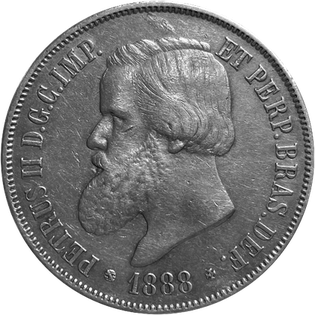
\includegraphics[width=2.0cm]{moeda-cara.png}};
        \node[jogador] (B1) at (-1.45,0) {$B$};
        \node[jogador] (A1) at (3.45,0) {$A$};
        \draw[->, teal!85!black, line width=0.9pt]
          (B1.east) -- (A1.west)
          node[midway, above=3pt, font=\small, text=teal!85!black] {$\mathrm{R\$}~1$};
      \end{scope}

      % Coroa: o jogador A paga R$ 1 ao jogador B.
      \begin{scope}[yshift=-1.25cm]
        \node[anchor=east, font=\footnotesize, text=text] at (-4.20,0) {coroa $(q)$};
        \node at (-3.10,0) {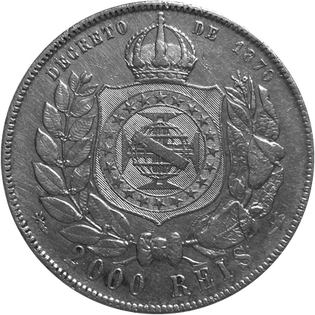
\includegraphics[width=2.0cm]{moeda-coroa.png}};
        \node[jogador] (A2) at (-1.45,0) {$A$};
        \node[jogador] (B2) at (3.45,0) {$B$};
        \draw[->, teal!85!black, line width=0.9pt]
          (A2.east) -- (B2.west)
          node[midway, above=3pt, font=\small, text=teal!85!black] {$\mathrm{R\$}~1$};
      \end{scope}

    \end{scope}

  \end{tikzpicture}
  \caption{Regra de pagamento em cada lançamento da moeda. Se o resultado é
    cara, o jogador $B$ entrega $\mathrm{R\$}~1$ ao jogador $A$; se é coroa,
    é o jogador $A$ quem entrega $\mathrm{R\$}~1$ ao jogador $B$. A moeda é
    uma peça de 2000 réis de 1888, com a efígie de D.~Pedro~II em uma face e a
    coroa imperial no verso.}
  \label{fig:pagamento-cara-coroa}
\end{figure}

Para modelar a evolução do capital dos jogadores durante esta partida,
basta acompanharmos o capital do jogador A após cada
lançamento. A sequência resultante de capitais é um passeio aleatório simples
sobre o conjunto finito $\{0, 1, \ldots, N\}$, iniciado no ponto $a$, que segue
suas transições usuais até atingir $0$ ou $N$, instante em que o processo é
interrompido. Dizemos que $0$ e $N$ são \emph{barreiras absorventes}, pois, uma
vez atingido qualquer um desses extremos, o passeio permanece nele. Dizemos
também que A \emph{vence o jogo} se o passeio é absorvido em $N$, e que B
\emph{vence o jogo} se o passeio é absorvido em $0$ (veja
\Cref{fig:barreiras-absorventes}). Como veremos nos
\cref{exercise:termino-ruina,exercise:vitoria-b}, a probabilidade de o jogo
continuar indefinidamente é zero, de modo que, quase certamente, exatamente um
dos jogadores vence. Qual é, então, a probabilidade de o jogador A vencer o
jogo?

\begin{figure}[htbp]
  \centering
  \begin{tikzpicture}[
    x=0.68cm, y=0.45cm,
    >=Stealth,
    font=\small,
  ]
    % Faixa do espaco de estados {0, ..., N}
    \fill[teal!6] (0, 0) rectangle (16, 10);

    % Grade horizontal leve para os estados intermediarios
    \foreach \y in {2, 4, 6, 8} {
      \draw[black!14, densely dashed, line width=0.4pt] (0, \y) -- (16, \y);
    }

    % Barreiras absorventes em 0 e N
    \draw[muted, densely dashed, line width=0.8pt] (0, 0) -- (16.4, 0);
    \draw[teal!85!black, densely dashed, line width=0.8pt] (0, 10) -- (16.4, 10);

    % Eixos
    \draw[->, black!65, line width=0.6pt] (0, -0.5) -- (0, 11.2)
      node[above=2pt, font=\small, text=text] {$S_n$};
    \draw[->, black!65, line width=0.6pt] (-0.3, 0) -- (16.8, 0)
      node[right=2pt, font=\small, text=text] {$n$};

    % Rotulos no eixo vertical
    \node[left=3pt, font=\scriptsize, text=muted] at (0, 0) {$0$};
    \node[left=3pt, font=\scriptsize, text=text] at (0, 4) {$a$};
    \node[left=3pt, font=\scriptsize, text=teal!85!black] at (0, 10) {$N$};

    % Trajetoria de exemplo partindo de a=4 ate absorcao em N=10 no passo 12
    \draw[teal, line width=1.35pt]
      (0, 4) -- (1, 5) -- (2, 4) -- (3, 5) -- (4, 6) -- (5, 7) -- (6, 6)
      -- (7, 7) -- (8, 8) -- (9, 7) -- (10, 8) -- (11, 9) -- (12, 10);
    % Permanencia na barreira absorvente
    \draw[teal, line width=1.35pt, dotted] (12, 10) -- (15.5, 10);

    % Marcadores nos pontos da trajetoria
    \foreach \x/\y in {0/4, 1/5, 2/4, 3/5, 4/6, 5/7, 6/6, 7/7, 8/8, 9/7, 10/8, 11/9} {
      \fill[teal] (\x, \y) circle (1.7pt);
    }
    % Ponto de absorcao destacado
    \fill[teal!85!black] (12, 10) circle (2.6pt);
    \draw[black!45, densely dashed, line width=0.45pt] (12, 0) -- (12, 10);
    \node[below=2pt, font=\scriptsize, text=text] at (12, 0) {$F$};

    % Anotacoes das barreiras
    \node[above=2pt, font=\scriptsize, text=teal!85!black, anchor=south east] at (16.2, 10)
      {barreira absorvente $N$ (vitória de A)};
    \node[below=10pt, font=\scriptsize, text=muted, anchor=north east] at (16.2, 0)
      {barreira absorvente $0$ (vitória de B)};
  \end{tikzpicture}
  \caption{Trajetória de um passeio aleatório simples em $\{0, 1, \ldots, N\}$
    partindo de $a$ até ser absorvido na barreira $N$ no instante $F$. Após
    atingir $0$ ou $N$, o passeio permanece constante na respectiva barreira.}
  \label{fig:barreiras-absorventes}
\end{figure}

Para responder a essa pergunta, usaremos um fato sobre probabilidades
condicionais que ainda não apareceu no curso: a aplicação
$E \mapsto \mathbb{P}(E \mid C)$ é ela própria uma medida de probabilidade, e
condicioná-la a um evento $D$ equivale a condicionar $\mathbb{P}$ à interseção
$C \cap D$. Escrevemos $\mathbb{P}(E \mid C, D)$ para denotar
$\mathbb{P}(E \mid C \cap D)$. Provamos este fato no lema a seguir.

\begin{lemma}[Condicionar uma probabilidade condicional]\label{lem:condicional}
  Seja $(\Omega, \mathcal{F}, \mathbb{P})$ um espaço de probabilidade, seja
  $C \in \mathcal{F}$ com $\mathbb{P}(C) > 0$ e defina
  \[
    \mathbb{Q}(E) \equiv \mathbb{P}(E \mid C), \qquad E \in \mathcal{F}.
  \]
  Então $\mathbb{Q}$ é uma medida de probabilidade em $(\Omega, \mathcal{F})$
  e, para todo $D \in \mathcal{F}$ com $\mathbb{Q}(D) > 0$,
  \[
    \mathbb{Q}(E \mid D) = \mathbb{P}(E \mid C \cap D)
    \qquad \text{para todo } E \in \mathcal{F}.
  \]
\end{lemma}

\begin{proof}
  A primeira afirmação segue direto da definição: $\mathbb{Q}(\varnothing) = 0$,
  $\mathbb{Q}(\Omega) = 1$ e, se $(E_n)_{n \geqslant 1}$ são eventos dois a
  dois disjuntos, então
  \[
    \mathbb{Q}\Bigl(\bigcup_{n \geqslant 1} E_n\Bigr)
    = \frac{\mathbb{P}\bigl(\bigcup_{n \geqslant 1} E_n \cap C\bigr)}{\mathbb{P}(C)}
    = \sum_{n \geqslant 1} \frac{\mathbb{P}(E_n \cap C)}{\mathbb{P}(C)}
    = \sum_{n \geqslant 1} \mathbb{Q}(E_n),
  \]
  em que a segunda igualdade usa a aditividade de $\mathbb{P}$.

  Para a segunda afirmação, pela definição de probabilidade condicional
  aplicada à medida $\mathbb{Q}$,
  \[
    \mathbb{Q}(E \mid D)
    = \frac{\mathbb{Q}(E \cap D)}{\mathbb{Q}(D)}
    = \frac{\mathbb{P}(E \cap D \mid C)}{\mathbb{P}(D \mid C)}
    = \frac{\mathbb{P}(E \cap D \cap C)}{\mathbb{P}(D \cap C)}
    = \mathbb{P}(E \mid C \cap D),
  \]
  o que conclui a demonstração.
\end{proof}

Com a definições e os resultados preliminares em mãos podemos provar o seguinte
resultado.

\begin{theorem}[Ruína do Jogador]\label{thm:ruina-probabilidade}
  Considere um passeio aleatório simples sobre $\{0, 1, \ldots, N\}$ com
  barreiras absorventes em $0$ e $N$. Se o passeio começa no ponto $a$, com
  $0 \leqslant a \leqslant N$, então a probabilidade de o jogador A vencer o
  jogo, dado que seu capital inicial é $\mathrm{R\$}~a$, é
  \begin{equation}\label{eq:ruina-v}
    v(a) \equiv \mathbb{P}(\text{A vence} \mid S_0 = a) =
    \begin{cases}
      \dfrac{(q/p)^a - 1}{(q/p)^N - 1}, & \text{se } p \neq q, \\[0.35cm]
      \dfrac{a}{N}, & \text{se } p = q = \tfrac{1}{2}.
    \end{cases}
  \end{equation}
\end{theorem}

\begin{proof}
  Para cada $0 \leqslant a \leqslant N$, seja
  $v(a) = \mathbb{P}(\text{A vence} \mid S_0 = a)$. Se
  $a = 0$, o jogador A já perdeu, logo $v(0) = 0$; se $a = N$, o jogador A já
  venceu, logo $v(N) = 1$.

  Suponha agora que $1 \leqslant a \leqslant N - 1$ e seja $H$ o evento em que
  o primeiro lançamento da moeda resulta em cara. Fixado esse $a$, seja
  \[
    \mathbb{Q}(E) \equiv \mathbb{P}(E \mid S_0 = a), \qquad E \in \mathcal{F}.
  \]
  Pelo \Cref{lem:condicional}, $\mathbb{Q}$ é uma medida de probabilidade e
  \[
    \mathbb{Q}(E \mid D) = \mathbb{P}(E \mid S_0 = a, D)
  \]
  para todo evento $D$ com $\mathbb{Q}(D) > 0$. Como
  $v(a) = \mathbb{Q}(\text{A vence})$, o Teorema da Partição aplicado a
  $\mathbb{Q}$ e à partição $\{H, H^c\}$ fornece
  \begin{align*}
    v(a)
    &= \mathbb{Q}(\text{A vence}) \\
    &= \mathbb{Q}(\text{A vence} \mid H)\,\mathbb{Q}(H)
     + \mathbb{Q}(\text{A vence} \mid H^c)\,\mathbb{Q}(H^c).
  \end{align*}

  Resta identificar os quatro fatores. Como o resultado do primeiro lançamento
  não depende do capital inicial,
  $\mathbb{Q}(H) = \mathbb{P}(H \mid S_0 = a) = p$ e
  $\mathbb{Q}(H^c) = \mathbb{P}(H^c \mid S_0 = a) = q$. Quando $H$ ocorre, o
  capital do jogador A passa de $\mathrm{R\$}~a$ para $\mathrm{R\$}~(a + 1)$
  após o primeiro lançamento; como os lançamentos subsequentes são
  independentes do primeiro e têm a mesma distribuição, 
  o processo evoluiu como se estivéssemos começando o jogo com o 
  jogador $A$ tendo capital inicial igual $\mathrm{R\$}~(a + 1)$. 
  Usando novamente o \Cref{lem:condicional} podemos concluir que
  \[ \mathbb{Q}(\text{A vence} \mid H)
   = \mathbb{P}(\text{A vence} \mid S_0 = a, H) = v(a + 1).
   \] 
  De modo análogo,
  quando $H^c$ ocorre o capital cai para $\mathrm{R\$}~(a - 1)$ e
  $\mathbb{Q}(\text{A vence} \mid H^c) = v(a - 1)$.

  Substituindo essas identidades na fórmula da partição, obtemos a equação de
  diferenças
  \begin{equation}\label{eq:ruina-dif-v}
    v(a) = p\,v(a + 1) + q\,v(a - 1), \qquad 1 \leqslant a \leqslant N - 1,
  \end{equation}
  sujeita às condições de contorno $v(0) = 0$ e $v(N) = 1$.

  Para resolver \eqref{eq:ruina-dif-v}, usamos $p + q = 1$ para escrever
  $v(a) = p\,v(a) + q\,v(a)$ e reorganizar a recorrência na forma
  \[
    p\bigl(v(a + 1) - v(a)\bigr) = q\bigl(v(a) - v(a - 1)\bigr),
    \qquad 1 \leqslant a \leqslant N - 1.
  \]
  Como $p > 0$, segue que
  \[
    v(a + 1) - v(a) = \frac{q}{p}\bigl(v(a) - v(a - 1)\bigr),
    \qquad 1 \leqslant a \leqslant N - 1.
  \]
  Aplicando essa relação recursivamente a partir de $k = 0$ e lembrando que
  $v(0) = 0$, obtemos, para todo $k \in \{0, 1, \ldots, N - 1\}$,
  \[
    v(k + 1) - v(k) = \left(\frac{q}{p}\right)^k \bigl(v(1) - v(0)\bigr)
    = \left(\frac{q}{p}\right)^k v(1).
  \]
  Somando telescopicamente de $k = 0$ até $a - 1$, encontramos, para todo
  $1 \leqslant a \leqslant N$,
  \[
    v(a) = v(a) - v(0)
    = \sum_{k=0}^{a-1} \bigl(v(k + 1) - v(k)\bigr)
    = v(1) \sum_{k=0}^{a-1} \left(\frac{q}{p}\right)^k.
  \]

  Resta avaliar essa soma nos dois casos possíveis. Se $p = q = \tfrac{1}{2}$,
  então $q/p = 1$ e a soma vale $a$, donde $v(a) = a\,v(1)$. Como $v(N) = 1$,
  temos $N\,v(1) = 1$, isto é, $v(1) = 1/N$, e portanto $v(a) = a/N$ (fórmula
  que também vale para $a = 0$).

  Se $p \neq q$, então $q/p \neq 1$, e a soma geométrica fornece
  \[
    v(a) = v(1)\,\frac{(q/p)^a - 1}{(q/p) - 1},
    \qquad 1 \leqslant a \leqslant N.
  \]
  Impondo a condição de contorno $v(N) = 1$, obtemos
  \[
    1 = v(1)\,\frac{(q/p)^N - 1}{(q/p) - 1},
    \qquad \text{logo} \qquad
    v(1) = \frac{(q/p) - 1}{(q/p)^N - 1}.
  \]
  Substituindo esse valor de $v(1)$ na expressão de $v(a)$, concluímos que
  \[
    v(a) = \frac{(q/p)^a - 1}{(q/p)^N - 1}
  \]
  para todo $0 \leqslant a \leqslant N$ (incluindo $a = 0$, em que o numerador
  se anula). Isso completa a demonstração.
\end{proof}

Outro cálculo clássico envolvendo equações de diferenças no Problema da Ruína
do Jogador diz respeito à duração esperada da partida. Novamente, formulamos o
resultado em termos do passeio aleatório associado.

\begin{theorem}[Tempo Esperado de Absorção]\label{thm:ruina-duracao}
  Considere um passeio aleatório simples sobre $\{0, 1, \ldots, N\}$ com
  barreiras absorventes em $0$ e $N$. Se o passeio começa no ponto $a$, com
  $0 \leqslant a \leqslant N$, então o número esperado $e(a)$ de passos até que
  o passeio seja absorvido em $0$ ou em $N$ é dado por
  \begin{equation}\label{eq:ruina-e}
    e(a) =
    \begin{cases}
      \dfrac{1}{p - q}
      \left( N\,\dfrac{(q/p)^a - 1}{(q/p)^N - 1} - a \right),
      & \text{se } p \neq q, \\[0.4cm]
      a(N - a), & \text{se } p = q = \tfrac{1}{2}.
    \end{cases}
  \end{equation}
\end{theorem}

Portanto, o número esperado de lançamentos da moeda até que A ou B vá à ruína
é dado por \eqref{eq:ruina-e}.

\begin{proof}
Seja $F$ o número de lançamentos da moeda até o término do jogo, de modo que
$e(a) = \mathbb{E}[F]$ quando o passeio parte de $a$. Observemos primeiro que
$e(a) < \infty$ para todo $0 \leqslant a \leqslant N$. De fato, se dividirmos
os lançamentos em blocos disjuntos de comprimento $N$, cada bloco consiste
exclusivamente de caras com probabilidade $p^N > 0$, evento que garante que o
passeio atinja $N$ caso ainda não tenha sido absorvido. Assim, para qualquer
estado inicial $a$ e todo $k \geqslant 0$, vale
$\mathbb{P}(F > kN) \leqslant (1 - p^N)^k$. Para transportar essa estimativa
ao valor esperado, usamos a fórmula da cauda e agrupamos os índices $n$ em
blocos de $N$ termos consecutivos. Como a sequência
$n \mapsto \mathbb{P}(F > n)$ é não crescente, todos os termos do bloco
$\{kN, kN + 1, \ldots, kN + N - 1\}$ são majorados por
$\mathbb{P}(F > kN)$, donde
\begin{align*}
  \mathbb{E}[F]
  &= \sum_{n=0}^{\infty} \mathbb{P}(F > n)
   = \sum_{k=0}^{\infty} \sum_{j=0}^{N-1} \mathbb{P}(F > kN + j)
  \\
  &\leqslant \sum_{k=0}^{\infty} N\,(1 - p^N)^k
   = \frac{N}{p^N} < \infty.
\end{align*}
Essa finitude assegura que todas as esperanças abaixo estão bem definidas e
podem ser manipuladas algebricamente.

Para $a = 0$ ou $a = N$, o jogo já está encerrado no instante inicial, logo
$e(0) = e(N) = 0$. Suponha agora que $1 \leqslant a \leqslant N - 1$ e seja
$H$ o evento em que o primeiro lançamento mostra cara. Pelo Teorema da
Partição para esperanças, temos
\[
e(a) = \mathbb{E}[F]
= \mathbb{E}[F \mid H]\,\mathbb{P}(H)
+ \mathbb{E}[F \mid H^c]\,\mathbb{P}(H^c).
\]
Se $H$ ocorre, o capital do jogador A sobe para $\mathrm{R\$}~(a + 1)$ após
o primeiro lançamento, logo $\mathbb{E}[F \mid H] = 1 + e(a + 1)$, em que a
parcela $1$ contabiliza o primeiro lançamento e $e(a + 1)$ é o número médio
de lançamentos subsequentes. Analogamente,
$\mathbb{E}[F \mid H^c] = 1 + e(a - 1)$. A relação acima torna-se então
\[
e(a) = \bigl(1 + e(a + 1)\bigr)p + \bigl(1 + e(a - 1)\bigr)q.
\]
Como $p + q = 1$, podemos reescrever essa identidade como a equação de
diferenças não homogênea
\begin{equation}\label{eq:ruina-dif-e}
p\,e(a + 1) - e(a) + q\,e(a - 1) = -1,
\qquad 1 \leqslant a \leqslant N - 1,
\end{equation}
sujeita às condições de contorno $e(0) = e(N) = 0$.

Para resolver \eqref{eq:ruina-dif-e}, reduzimos o problema à equação
homogênea já resolvida na demonstração do \Cref{thm:ruina-probabilidade}
subtraindo uma solução particular explícita.

\smallskip
\noindent\textbf{Caso 1: $p \neq q$.}
A função $a \mapsto -a/(p - q)$ é uma solução particular de
\eqref{eq:ruina-dif-e}, pois $p + q = 1$ implica
\[
p\left(-\frac{a + 1}{p - q}\right)
- \left(-\frac{a}{p - q}\right)
+ q\left(-\frac{a - 1}{p - q}\right)
= \frac{-p(a + 1) + (p + q)a - q(a - 1)}{p - q}
= \frac{q - p}{p - q} = -1.
\]
Defina $u(a) = e(a) + a/(p - q)$ para $0 \leqslant a \leqslant N$. Pela
linearidade da equação de diferenças, $u(a)$ satisfaz a equação homogênea
\[
p\,u(a + 1) - u(a) + q\,u(a - 1) = 0,
\qquad 1 \leqslant a \leqslant N - 1,
\]
com condições de contorno $u(0) = 0$ e $u(N) = N/(p - q)$. Pelo argumento
telescópico da demonstração do \Cref{thm:ruina-probabilidade}, toda solução
dessa equação homogênea com valor nulo em $0$ é proporcional a $v(a)$, ou
seja,
\[
u(a) = u(N)\,v(a)
= \frac{N}{p - q}\,\frac{(q/p)^a - 1}{(q/p)^N - 1},
\qquad 0 \leqslant a \leqslant N.
\]
Subtraindo $a/(p - q)$, obtemos a primeira linha de \eqref{eq:ruina-e}.

\smallskip
\noindent\textbf{Caso 2: $p = q = \tfrac{1}{2}$.}
Nesse caso, a equação \eqref{eq:ruina-dif-e} admite a solução particular
$a \mapsto -a^2$, já que
\[
\frac{1}{2}\bigl(-(a + 1)^2\bigr) - (-a^2) + \frac{1}{2}\bigl(-(a - 1)^2\bigr)
= -\frac{a^2 + 2a + 1 - 2a^2 + a^2 - 2a + 1}{2} = -1.
\]
Definindo $u(a) = e(a) + a^2$, obtemos novamente uma solução da equação
homogênea $\tfrac{1}{2}u(a + 1) - u(a) + \tfrac{1}{2}u(a - 1) = 0$, agora com
$u(0) = 0$ e $u(N) = N^2$. Como qualquer solução dessa equação com $u(0) = 0$
é da forma $u(a) = a\,u(1)$, a condição em $N$ dá $u(1) = N$, logo
$u(a) = Na$. Consequentemente, $e(a) = Na - a^2 = a(N - a)$, o que conclui a
demonstração.
\end{proof}

A \Cref{fig:curvas-ruina} ilustra o comportamento de $v(a)$ e $e(a)$ para
$N = 20$ em três regimes de probabilidade: o caso simétrico ($p = 0{,}5$) e
dois casos assimétricos ($p = 0{,}45$ e $p = 0{,}55$). Observa-se como uma
pequena vantagem ou desvantagem por lançamento altera fortemente a
probabilidade de vitória de A e desloca o ponto de máxima duração esperada do
jogo.

\begin{figure}[htbp]
  \centering
  \begin{tikzpicture}[font=\small]
    \begin{axis}[
      name=leftplot,
      width=7.1cm,
      height=5.4cm,
      xmin=0, xmax=20,
      ymin=0, ymax=1.05,
      xlabel={$a$},
      ylabel={$v(a)$},
      title={Probabilidade de vitória de A},
      title style={font=\small, text=text},
      axis lines=left,
      grid=major,
      grid style={black!14, densely dashed, line width=0.4pt},
      tick label style={font=\scriptsize, text=muted},
      label style={font=\small, text=text},
      /pgf/number format/use comma,
      legend style={
        at={(0.97, 0.05)},
        anchor=south east,
        font=\scriptsize,
        draw=border,
        fill=white,
        fill opacity=0.9,
        text opacity=1,
        cells={anchor=west},
      },
    ]
      % p = 0.55 (q/p = 9/11)
      \addplot[
        color=text,
        dashed,
        line width=1.05pt,
        domain=0:20,
        samples=21,
      ] {((9/11)^x - 1)/((9/11)^20 - 1)};
      \addlegendentry{$p = 0{,}55$}

      % p = 0.50
      \addplot[
        teal,
        line width=1.35pt,
        domain=0:20,
        samples=21,
      ] {x/20};
      \addlegendentry{$p = 0{,}50$}

      % p = 0.45 (q/p = 11/9)
      \addplot[
        muted,
        densely dotted,
        line width=1.15pt,
        domain=0:20,
        samples=21,
      ] {((11/9)^x - 1)/((11/9)^20 - 1)};
      \addlegendentry{$p = 0{,}45$}
    \end{axis}

    \begin{axis}[
      at={(leftplot.outer south east)},
      anchor=outer south west,
      xshift=0.7cm,
      width=7.1cm,
      height=5.4cm,
      xmin=0, xmax=20,
      ymin=0, ymax=108,
      xlabel={$a$},
      ylabel={$e(a)$},
      title={Duração esperada do jogo},
      title style={font=\small, text=text},
      axis lines=left,
      grid=major,
      grid style={black!14, densely dashed, line width=0.4pt},
      tick label style={font=\scriptsize, text=muted},
      label style={font=\small, text=text},
      /pgf/number format/use comma,
      legend style={
        at={(0.97, 0.97)},
        anchor=north east,
        font=\scriptsize,
        draw=border,
        fill=white,
        fill opacity=0.9,
        text opacity=1,
        cells={anchor=west},
      },
    ]
      % p = 0.50
      \addplot[
        teal,
        line width=1.35pt,
        domain=0:20,
        samples=21,
      ] {x*(20 - x)};
      \addlegendentry{$p = 0{,}50$}

      % p = 0.55 (p - q = 0.1)
      \addplot[
        color=text,
        dashed,
        line width=1.05pt,
        domain=0:20,
        samples=21,
      ] {10*(20*((9/11)^x - 1)/((9/11)^20 - 1) - x)};
      \addlegendentry{$p = 0{,}55$}

      % p = 0.45 (p - q = -0.1)
      \addplot[
        muted,
        densely dotted,
        line width=1.15pt,
        domain=0:20,
        samples=21,
      ] {-10*(20*((11/9)^x - 1)/((11/9)^20 - 1) - x)};
      \addlegendentry{$p = 0{,}45$}
    \end{axis}
  \end{tikzpicture}
  \caption{Curvas da probabilidade de vitória $v(a)$ e da duração esperada
    $e(a)$ no Problema da Ruína do Jogador com capital total $N = 20$. À
    esquerda, $v(a)$ é linear quando $p = 0{,}50$ (linha contínua), côncava
    quando $p = 0{,}55$ (tracejada) e convexa quando $p = 0{,}45$ (pontilhada).
    À direita, $e(a)$ atinge o máximo $100$ em $a = 10$ no caso simétrico e
    torna-se assimétrica quando $p \neq 0{,}50$.}
  \label{fig:curvas-ruina}
\end{figure}

Por fim, o que acontece com as chances do jogador A quando seu adversário é
infinitamente rico? Embora essa situação não ocorra literalmente na prática,
esse modelo idealizado ajuda a compreender o comportamento de longo prazo de um
apostador diante de um cassino com reservas muito grandes. Nesse cenário, A
jamais pode derrotar o oponente, mas pode ao menos esperar escapar da falência
definitiva e continuar jogando para sempre. A probabilidade de que A acabe
levado à ruína é dada pelo teorema final sobre passeios aleatórios
unidimensionais.

\begin{theorem}[Ruína Contra Adversário Infinitamente Rico]\label{thm:ruina-infinito}
  Considere um passeio aleatório simples sobre $\{0, 1, 2, \ldots\}$ com uma
  barreira absorvente em $0$. Se o passeio começa no ponto $a \geqslant 0$,
  então a probabilidade $\pi(a)$ de que o passeio seja eventualmente absorvido
  em $0$ é dada por
  \begin{equation}\label{eq:ruina-pi}
    \pi(a) =
    \begin{cases}
      \left(\dfrac{q}{p}\right)^a, & \text{se } p > q, \\[0.3cm]
      1, & \text{se } p \leqslant q.
    \end{cases}
  \end{equation}
\end{theorem}

Com capital inicial $a > 0$, o jogador A tem probabilidade positiva de jogar
indefinidamente se, e somente se, $p > q$, o que justifica \eqref{eq:ruina-exemplo}.
Na \Cref{rem:ruina-limite}, obtemos a mesma fórmula a partir do jogo finito,
mantendo fixo o capital inicial $a$ de A e fazendo o capital total $N$ tender
a infinito.

\begin{proof}
  Se $a = 0$, o passeio já está absorvido, logo $\pi(0) = 1$. Para
  $a \geqslant 1$, o capital sobe para $a + 1$ com probabilidade $p$ ou cai
  para $a - 1$ com probabilidade $q$ no primeiro lançamento. Como os
  lançamentos seguintes são independentes do primeiro, a probabilidade de
  ruína em cada caso é a de um jogo que começa com o novo capital.
  Condicionando no primeiro lançamento, como em \eqref{eq:ruina-dif-v}, obtemos
  \[
    \pi(a) = p\,\pi(a + 1) + q\,\pi(a - 1), \qquad a = 1, 2, \ldots.
  \]
  Como no \Cref{thm:ruina-probabilidade}, usamos $p + q = 1$ para escrever
  a recorrência em termos das diferenças entre valores consecutivos de $\pi$.
  Com $r = q/p$, temos
  \[
    \pi(a + 1) - \pi(a) = r\bigl(\pi(a) - \pi(a - 1)\bigr),
    \qquad a = 1, 2, \ldots.
  \]
  Cada diferença é $r$ vezes a anterior. Assim, a primeira diferença
  $\pi(1) - 1$ determina todas as demais, com
  $\pi(k + 1) - \pi(k) = r^k\bigl(\pi(1) - 1\bigr)$ para $k \geqslant 0$.
  Recuperamos $\pi(a)$ somando essas diferenças a partir de $\pi(0)$.
  A soma é telescópica e, para $a \geqslant 1$, dá
  \begin{equation}\label{eq:ruina-pi-geral}
    \pi(a) = \pi(0) + \sum_{k=0}^{a-1} \bigl(\pi(k + 1) - \pi(k)\bigr)
    = 1 + \bigl(\pi(1) - 1\bigr) \sum_{k=0}^{a-1} r^k.
  \end{equation}

  No jogo finito, a condição de contorno na barreira $N$ fixava a primeira
  diferença. Aqui, a única barreira é $0$, e a condição $\pi(0) = 1$ já foi
  usada. Podemos ainda exigir que \eqref{eq:ruina-pi-geral} tome valores entre
  $0$ e $1$ para todo $a$. O que essa restrição nos diz sobre $\pi(1)$ depende
  de como a soma geométrica se comporta quando $a$ cresce.

  \smallskip
  \noindent\textbf{Caso $p \leqslant q$.}
  Como $r \geqslant 1$, cada parcela da soma em \eqref{eq:ruina-pi-geral}
  é pelo menos $1$, de modo que a soma cresce sem limite com $a$. Se
  $\pi(1) < 1$, o coeficiente $\pi(1) - 1$ é negativo e a fórmula acabaria
  dando $\pi(a) < 0$ para $a$ suficientemente grande. Portanto, $\pi(1) = 1$.
  Substituindo em \eqref{eq:ruina-pi-geral}, concluímos que
  \begin{equation}\label{eq:ruina-certa}
    \text{se } p \leqslant q, \qquad \pi(a) = 1 \quad
    \text{para todo } a \geqslant 0.
  \end{equation}

  \smallskip
  \noindent\textbf{Caso $p > q$.}
  Agora $0 < r < 1$, e a soma em \eqref{eq:ruina-pi-geral} é limitada por
  $1/(1 - r)$. Para qualquer escolha de $\pi(1)$ em $[r, 1]$, temos
  $0 \leqslant 1 - \pi(1) \leqslant 1 - r$. Multiplicando pela soma,
  vemos que a quantidade subtraída de $1$ em \eqref{eq:ruina-pi-geral} fica
  entre $0$ e $1$. Logo, toda escolha nesse intervalo é compatível com a
  restrição $0 \leqslant \pi(a) \leqslant 1$.

  Para determinar $\pi(1)$, podemos interpretar a ruína a partir de $1$
  como um retorno a $0$ após um primeiro passo para a direita. Essa
  interpretação permite usar a fórmula \eqref{eq:prob-retorno} do
  \Cref{thm:recorrencia-transiencia}.

  Considere então um passeio aleatório simples $(T_n)_{n \geqslant 0}$ em
  $\mathbb{Z}$ com os mesmos parâmetros $p$ e $q$, iniciado em $T_0 = 0$, e
  seja $C = \{T_n = 0 \text{ para algum } n \geqslant 1\}$ o evento de
  retorno à origem. Como $T_1$ vale $1$ ou $-1$, o retorno só pode ocorrer
  a partir do instante $2$.

  Para ler a trajetória a partir do instante $1$, escrevemos
  $X_j = T_j - T_{j-1}$ para o deslocamento no passo $j$. Pela representação
  \eqref{eq:passeio-soma}, temos
  \[
    T_{m+1} = T_1 + \sum_{j=2}^{m+1} X_j, \qquad m = 0, 1, 2, \ldots.
  \]
  Nessa expressão, $T_1$ é a posição inicial do trecho que começa depois do
  primeiro passo, e $m$ conta os passos a partir dali. Como $T_1 = X_1$ e os
  incrementos são independentes, sob cada uma das condições $T_1 = 1$ e
  $T_1 = -1$, os deslocamentos $X_2, X_3, \ldots$ continuam independentes e
  cada um vale $1$ com probabilidade $p$ e $-1$ com probabilidade $q$.

  \smallskip
  \noindent\textit{Primeiro passo para a direita $(T_1 = 1)$.}
  O trecho parte de $1$ e permanece nos inteiros positivos até a primeira
  visita a $0$, pois cada passo tem tamanho $1$. Se a trajetória atinge $0$,
  podemos mantê-la ali de então em diante para obter o jogo com capital
  inicial $1$ e barreira absorvente em $0$. A primeira visita a $0$ é ao
  mesmo tempo o retorno do passeio original e o instante da ruína no jogo.
  Portanto,
  \[
    \mathbb{P}(C \mid T_1 = 1) = \pi(1).
  \]

  \smallskip
  \noindent\textit{Primeiro passo para a esquerda ($T_1 = -1$).}
  Para aproveitar \eqref{eq:ruina-certa}, que trata de capital inicial
  positivo, refletimos a trajetória pela transformação $x \mapsto -x$.
  O trecho refletido começa em $-T_1 = 1$. Para $j \geqslant 2$, seu
  incremento no passo $j$ é $(-T_j) - (-T_{j-1}) = -X_j$. Logo, um passo
  para a esquerda no passeio original vira um passo para a direita no
  refletido, e vice-versa. Sob a condição $T_1 = -1$, temos
  \[
    \mathbb{P}(-X_j = 1 \mid T_1 = -1) = q,
    \qquad
    \mathbb{P}(-X_j = -1 \mid T_1 = -1) = p.
  \]
  Os passos refletidos continuam independentes, pois cada um é obtido
  trocando o sinal de um único incremento. Assim, até a primeira visita a
  $0$, o trecho refletido representa um jogo com capital inicial $1$, no
  qual o capital sobe com probabilidade $q$ e desce com probabilidade $p$.
  Como $q < p$, a probabilidade de subir é menor que a de descer, e
  \eqref{eq:ruina-certa} dá probabilidade de ruína igual a $1$ para esse
  jogo. Em cada instante, temos $-T_n = 0$ exatamente quando $T_n = 0$.
  Portanto, a ruína do passeio refletido corresponde ao retorno do passeio
  original, e
  \[
    \mathbb{P}(C \mid T_1 = -1) = 1.
  \]

  Aplicando o Teorema da Partição aos eventos $\{T_1 = 1\}$ e $\{T_1 = -1\}$,
  como na dedução de \eqref{eq:ruina-dif-v} na prova do
  \Cref{thm:ruina-probabilidade}, obtemos
  \begin{equation}\label{eq:ruina-pi-pi1}
    \begin{aligned}
      \mathbb{P}(C)
      &= p\,\mathbb{P}(C \mid T_1 = 1) + q\,\mathbb{P}(C \mid T_1 = -1) \\
      &= p\,\pi(1) + q \cdot 1.
    \end{aligned}
  \end{equation}
  Por \eqref{eq:prob-retorno}, como $p > q$, também temos
  $\mathbb{P}(C) = 1 - (p - q) = 2q$. Comparando com \eqref{eq:ruina-pi-pi1},
  obtemos $p\,\pi(1) = q$ e, portanto, $\pi(1) = r$. Já sabemos que
  $\pi(0) = 1 = r^0$. Para $a \geqslant 1$, substituímos $\pi(1) = r$ em
  \eqref{eq:ruina-pi-geral} e avaliamos a soma geométrica.
  \[
    \pi(a) = 1 + (r - 1)\frac{1 - r^a}{1 - r} = r^a
    = \left(\frac{q}{p}\right)^a. \qedhere
  \]
\end{proof}

\begin{remark}[Justificativa rigorosa via limite $N \to \infty$]\label{rem:ruina-limite}
  Podemos deduzir \eqref{eq:ruina-pi} a partir do
  \Cref{thm:ruina-probabilidade} mantendo fixo o capital inicial de A e
  aumentando o de B. Para comparar os jogos, usamos a mesma sequência de
  lançamentos em todos eles. Assim, para cada trajetória podemos perguntar
  se A chegaria à ruína antes que o jogo terminasse na barreira superior.

  Se $a = 0$, o jogador A já começa na ruína, logo $\pi(0) = 1$. Fixe agora
  um inteiro $a \geqslant 1$. Sejam $X_1, X_2, \ldots$ os incrementos dos
  lançamentos, independentes, iguais a $1$ com probabilidade $p$ e a $-1$
  com probabilidade $q$. Como em \eqref{eq:passeio-soma}, construímos o
  passeio em $\mathbb{Z}$ que começa em $a$ pela fórmula
  \[
    S_n^{(a)} = a + \sum_{j=1}^n X_j, \qquad n = 0, 1, 2, \ldots.
  \]
  A soma é vazia em $n = 0$, de modo que $S_0^{(a)} = a$. Para cada
  $b \in \mathbb{Z}$, escrevemos $\tau_b^{(a)}$ para o primeiro instante
  $n \geqslant 0$ em que o passeio atinge $b$. Se $b$ nunca é atingido,
  tomamos $\tau_b^{(a)} = \infty$.

  No jogo contra o adversário infinitamente rico, A vai à ruína na
  primeira visita a $0$. Como o passeio começa em $a \geqslant 1$, essa
  visita, se ocorrer, será em algum instante $n \geqslant 1$. O evento de
  ruína é
  \[
    \begin{aligned}
      E^{(a)} &= \{\tau_0^{(a)} < \infty\} \\
              &= \{\text{existe } n \geqslant 1 \text{ tal que } S_n^{(a)} = 0\} \\
              &= \{\text{existe } n \geqslant 1 \text{ tal que } X_1 + \cdots + X_n = -a\}.
    \end{aligned}
  \]
  A última expressão mostra como o evento depende do capital inicial. Para
  levar o capital de A do valor inicial $a$ até zero, a soma dos incrementos
  precisa atingir $-a$. Pela definição de $\pi(a)$, temos
  $\mathbb{P}(E^{(a)}) = \pi(a)$.

  Para cada inteiro $N > a$, o jogo com capital inicial $N - a$ para B usa
  os mesmos lançamentos e termina na primeira visita a $0$ ou a $N$. Nesse
  jogo, o evento de ruína de A é
  \[
    E_N^{(a)} = \{\tau_0^{(a)} < \tau_N^{(a)}\}.
  \]
  O \Cref{thm:ruina-duracao} dá esperança finita para o tempo de absorção.
  Logo, o jogo termina com probabilidade $1$, pois um tempo infinito com
  probabilidade positiva teria esperança infinita. Assim, quase certamente,
  uma das duas barreiras é atingida primeiro. Se $v_N(a)$ denota a
  probabilidade de A vencer nesse jogo, dada por \eqref{eq:ruina-v}, então
  \[
    \mathbb{P}(E_N^{(a)}) = 1 - v_N(a).
  \]

  Ao passar de $N$ para $N + 1$, toda trajetória que atinge $0$ antes de
  $N$ também atinge $0$ antes de $N + 1$. Com efeito, partindo de $a < N$
  e dando passos de uma unidade, o passeio só chega a $N + 1$ depois de
  passar por $N$. Portanto, $E_N^{(a)} \subseteq E_{N+1}^{(a)}$.

  A união desses eventos contém exatamente as trajetórias em que A vai à
  ruína contra o adversário infinitamente rico. Se uma trajetória pertence a
  algum $E_N^{(a)}$, ela chega a $0$ em tempo finito e, portanto, pertence a
  $E^{(a)}$. Para a inclusão inversa, considere uma trajetória em $E^{(a)}$
  e seja $m$ o instante de sua primeira visita a $0$. A lista das posições
  registradas do instante $0$ ao instante $m$ tem $m + 1$ termos, de modo
  que existe um maior valor
  \[
    M = \max\{S_0^{(a)}, S_1^{(a)}, \ldots, S_m^{(a)}\}.
  \]
  Como $S_0^{(a)} = a$, temos $M \geqslant a$. Tomando $N = M + 1$,
  obtemos $N > a$ e garantimos que o passeio chega a $0$ no instante $m$
  antes de atingir $N$.
  Logo, essa trajetória pertence a $E_N^{(a)}$. A escolha de $N$ pode
  depender da trajetória, pois basta que ela pertença a um dos eventos da
  união. Concluímos que
  \[
    \bigcup_{N = a + 1}^{\infty} E_N^{(a)} = E^{(a)}.
  \]

  Por exemplo, uma trajetória que começa com as posições $2, 3, 2, 1, 0$
  pertence a $E_4^{(2)}$, pois chega a $0$ sem atingir $4$. Com a barreira
  em $3$, o jogo teria terminado no primeiro passo com a vitória de A.

  A passagem ao limite usa a continuidade da probabilidade por baixo.
  Como os eventos são crescentes, podemos decompor a união em partes
  disjuntas. A primeira é $E_{a+1}^{(a)}$ e cada uma das seguintes é
  $E_N^{(a)} \setminus E_{N-1}^{(a)}$, para $N \geqslant a + 2$. A soma
  das probabilidades dessas partes até a etapa $N$ vale
  $\mathbb{P}(E_N^{(a)})$. Ao incluir todas as partes, a aditividade
  enumerável dá a probabilidade da união. Portanto,
  \[
    \begin{aligned}
      \pi(a) &= \mathbb{P}(E^{(a)})
              = \mathbb{P}\left(\bigcup_{N = a + 1}^{\infty} E_N^{(a)}\right) \\
             &= \lim_{N \to \infty} \mathbb{P}(E_N^{(a)})
              = \lim_{N \to \infty} \bigl(1 - v_N(a)\bigr).
    \end{aligned}
  \]

  Para calcular o limite, mantemos $a$ fixo em \eqref{eq:ruina-v} e
  escrevemos $r = q/p$.
  \begin{itemize}
    \item Se $p = q$, então $v_N(a) = a/N \to 0$, logo $\pi(a) = 1$.
    \item Se $p < q$, então $r > 1$. O numerador $r^a - 1$ é constante e
    o denominador $r^N - 1$ tende a infinito, logo $v_N(a) \to 0$ e
    $\pi(a) = 1$.
    \item Se $p > q$, então $0 < r < 1$, de modo que $r^N \to 0$. Assim,
    $v_N(a) \to (r^a - 1)/(-1) = 1 - r^a$, logo $\pi(a) = r^a = (q/p)^a$.
  \end{itemize}
  Recuperamos, assim, a fórmula \eqref{eq:ruina-pi}.
\end{remark}

\begin{exercise}\label{exercise:termino-ruina}
  Mostre que, no Problema da Ruína do Jogador, o jogo termina com
  probabilidade $1$. Pode ser útil particionar a sequência de lançamentos da
  moeda em blocos disjuntos de comprimento $N$ e considerar o evento em que um
  desses blocos contém apenas passos para a direita.
\end{exercise}

\begin{exercise}\label{exercise:vitoria-b}
  Use o \Cref{thm:ruina-probabilidade} para mostrar que, no Problema da Ruína
  do Jogador, a probabilidade de que o jogador B vença o jogo é
  \[
    \mu(a) =
    \begin{cases}
      \dfrac{(p/q)^{N-a} - 1}{(p/q)^N - 1}, & \text{se } p \neq q, \\[0.35cm]
      \dfrac{N - a}{N}, & \text{se } p = q = \tfrac{1}{2},
    \end{cases}
  \]
  em que $\mathrm{R\$}~(N - a)$ é o capital inicial de B. Deduza que
  \[
    \mathbb{P}(\text{A vence}) + \mathbb{P}(\text{B vence}) = 1,
  \]
  e, portanto, que é nula a probabilidade de o jogo não terminar.
\end{exercise}

\begin{exercise}\label{exercise:capital-uniforme}
  Considere o Problema da Ruína do Jogador com a modificação de que o capital
  inicial do jogador A é distribuído uniformemente no conjunto
  $\{0, 1, 2, \ldots, N\}$. Qual é a probabilidade de que A vença o jogo?
\end{exercise}

\begin{exercise}\label{exercise:primeiro-passo-condicional}
  Considere o Problema da Ruína do Jogador com $0 < p < 1$ e
  $p \neq \tfrac{1}{2}$. Suponha que o capital inicial do jogador A seja
  $\mathrm{R\$}~k$, com $1 \leqslant k < N$, e que saibamos que A venceu o
  jogo. Qual é a probabilidade de que o primeiro passo tenha sido de $k$ para
  $k - 1$?
\end{exercise}

\section{Problemas}\label{sec:problemas}

Os problemas a seguir ampliam o que desenvolvemos nas seções anteriores,
explorando variantes de passeios aleatórios unidimensionais com barreiras,
passeios aleatórios em duas, três e $d$ dimensões, eventos recorrentes e
aplicações de funções geradoras de probabilidade. Não apresentamos soluções.
Em cada enunciado indicamos, quando isso não é evidente, qual resultado já
disponível deve ser empregado.

\providecommand{\starredproblem}{%
\refstepcounter{enumi}\llap{\textasteriskcentered\,}\arabic{enumi}.}

\begin{enumerate}[label={\arabic*.}]
\item\label{prob:duas-particulas-mesma-posicao}
Duas partículas realizam passeios aleatórios simétricos independentes e
simultâneos a partir da origem. Mostre que a probabilidade de que elas estejam
na mesma posição após $n$ passos é
\[
\left(\frac{1}{2}\right)^{2n}\sum_{k=0}^{n}\binom{n}{k}^2.
\]
A partir disso, ou por outro argumento, mostre que
\[
\sum_{k=0}^{n}\binom{n}{k}^2=\binom{2n}{n}.
\]

\item\label{prob:passeio-com-permanencia}
Considere um passeio aleatório nos inteiros com barreiras absorventes em $0$ e
$N$ no qual, a cada etapa, a partícula pode saltar uma unidade para a esquerda
(com probabilidade $\alpha$), permanecer onde está (com probabilidade $\beta$)
ou saltar uma unidade para a direita (com probabilidade $\gamma$), em que
$\alpha,\beta,\gamma>0$ e $\alpha+\beta+\gamma=1$. Se a partícula parte do
ponto $a$, com $0\leqslant a\leqslant N$, mostre que a probabilidade de ela ser
absorvida em $N$ é dada pela equação \eqref{eq:ruina-v} com
$p=1-q=\gamma/(\alpha+\gamma)$. Encontre o número médio de etapas até que a
partícula seja absorvida em uma das barreiras.

\item\label{prob:absorcao-antes-retorno}
Uma partícula realiza um passeio aleatório no conjunto
$\{-N,-N+1,\ldots,N-1,N\}$ e é absorvida se atingir $-N$ ou $N$, em que $N>1$.
A probabilidade de um passo de tamanho $-1$ é $q=1-p$, com $0<p<1$. Suponha
que a partícula parta de $0$. Condicionando no primeiro passo e usando o
\Cref{thm:ruina-probabilidade}, ou por outro método, mostre que, quando
$p\neq q$, a probabilidade de a partícula ser absorvida em $N$ ou $-N$ antes de
retornar a $0$ é
\[
\frac{(p-q)(p^N+q^N)}{p^N-q^N}.
\]
Qual é essa probabilidade quando $p=q$?

\smallskip
\noindent\emph{(Oxford, 1983)}

\item\label{prob:passeio-passos-2-menos-1}
Considere um passeio aleatório nos inteiros no qual a partícula se move duas
unidades para a direita (com probabilidade $p$) ou uma unidade para a esquerda
(com probabilidade $q=1-p$) a cada etapa, em que $0<p<1$. Há uma barreira
absorvente em $0$ e a partícula parte do ponto $a>0$. Mostre que a
probabilidade $\pi(a)$ de que a partícula seja eventualmente absorvida em $0$
satisfaz a equação de diferenças
\[
\pi(a)=p\pi(a+2)+q\pi(a-1), \qquad\text{para } a=1,2,\ldots,
\]
e deduza que $\pi(a)=1$ se $p\leqslant\tfrac{1}{3}$.

Suponha agora que a partícula também seja absorvida sempre que atingir $N$ ou
$N+1$. Encontre a probabilidade $\pi_N(a)$ de que ela seja absorvida em $0$, em
vez de em $N$ ou $N+1$, tendo partido de $a$, em que
$0\leqslant a\leqslant N+1$. Deduza que, quando $N\to\infty$,
\[
\pi_N(a)\to
\begin{cases}
1, & \text{se } p\leqslant\frac{1}{3}, \\[0.2cm]
\theta^a, & \text{se } p>\frac{1}{3},
\end{cases}
\]
em que $\theta=\frac{1}{2}\bigl[\sqrt{1+(4q/p)}-1\bigr]$.

Deduza que, se uma moeda honesta for lançada repetidamente, a probabilidade de
que o número de caras em algum momento exceda o dobro do número de coroas é
$\frac{1}{2}(\sqrt{5}-1)$.

\item\label{prob:barreira-retentora}
Considere um passeio aleatório simples com uma barreira absorvente em $0$ e uma
barreira ``retentora'' em $N$. Isto é, não é permitido ao passeio ultrapassar
$N$ à direita, de modo que sua posição $S_n$ no instante $n$ satisfaz
\[
\mathbb{P}(S_{n+1}=N\mid S_n=N)=p,
\qquad
\mathbb{P}(S_{n+1}=N-1\mid S_n=N)=q,
\]
em que $p+q=1$. Formule uma equação de diferenças para o número médio $e(a)$ de
saltos do passeio até a absorção em $0$, partindo de $a$, com
$0\leqslant a\leqslant N$. Deduza que
\[
e(a)=a(2N-a+1), \qquad\text{se } p=q=\frac{1}{2},
\]
e encontre $e(a)$ quando $p\neq q$.

\item\label{prob:numero-revisitas-assimetrico}
Seja $N$ o número de vezes em que um passeio aleatório simples assimétrico
revisita seu ponto de partida. Mostre que $N$ tem função de probabilidade dada
por
\[
\mathbb{P}(N=k)=\alpha(1-\alpha)^k, \qquad\text{para } k=0,1,2,\ldots,
\]
em que $\alpha=|p-q|$ e $p$ é a probabilidade de que cada passo do passeio seja
para a direita.

\item\label{prob:maquina-caca-niqueis}
Uma máquina caça-níqueis funciona da seguinte maneira. Na primeira jogada, o
jogador vence com probabilidade $\tfrac{1}{2}$. Nas jogadas seguintes, o
jogador vence com probabilidade $\tfrac{1}{2}$ se perdeu na jogada anterior e
com probabilidade $p<\tfrac{1}{2}$ se venceu. Mostre que a probabilidade $u_n$
de o jogador vencer na $n$-ésima jogada satisfaz
\[
u_n+\left(\frac{1}{2}-p\right)u_{n-1}=\frac{1}{2}, \qquad\text{para } n>1.
\]
Deduza que
\[
u_n=\frac{1+(-1)^{n-1}(\tfrac{1}{2}-p)^n}{3-2p}, \qquad\text{para } n\geqslant 1.
\]

\item\label{prob:passeio-2d-stirling}
Considere o passeio aleatório bidimensional do \Cref{exercise:passeio-2d}, no
qual uma partícula ocupa os pontos inteiros
$\{(i,j):i,j=\ldots,-1,0,1,\ldots\}$ do plano, movendo-se para a direita, para
cima, para a esquerda ou para baixo com respectivas probabilidades $p$, $q$, $r$
e $s$ a cada passo, em que $p,q,r,s>0$ e $p+q+r+s=1$. Seja $\mathbf{S}_n$ a
posição da partícula após $n$ passos, e suponha que $\mathbf{S}_0=(0,0)$. Seja
$v_n$ a probabilidade de que $\mathbf{S}_n=(0,0)$, e prove que
\[
v_{2m}=\binom{2m}{m}^2\left(\frac{1}{4}\right)^{2m},
\qquad\text{se } p=q=r=s=\frac{1}{4}.
\]
Use a Fórmula de Stirling para mostrar que
\[
\sum_{n=0}^{\infty}v_n=\infty,
\qquad\text{se } p=q=r=s=\frac{1}{4}.
\]
Deduza diretamente que o passeio aleatório simétrico em duas dimensões é
recorrente.

\item\label{prob:passeio-2d-rotacao}
Apresentamos aqui outra abordagem para o passeio aleatório simétrico em duas
dimensões do Problema~\ref{prob:passeio-2d-stirling}. Faça a seguinte mudança
de variáveis: se $\mathbf{S}_n=(i,j)$, defina $X_n=i+j$ e $Y_n=i-j$; isso
equivale a rotacionar os eixos por um ângulo de $\tfrac{1}{4}\pi$. Mostre que
$(X_n)_{n \geqslant 0}$ e $(Y_n)_{n \geqslant 0}$ são passeios aleatórios simétricos
independentes em uma dimensão. Deduza, pelo \Cref{thm:retorno-origem}, que
\[
\mathbb{P}(\mathbf{S}_{2m}=\mathbf{0}\mid\mathbf{S}_0=\mathbf{0})
=\left[\binom{2m}{m}\left(\frac{1}{2}\right)^{2m}\right]^2,
\]
em que $\mathbf{0}=(0,0)$.

\item\label{prob:passeio-2d-distancia}
No passeio aleatório bidimensional do Problema~\ref{prob:passeio-2d-stirling},
seja $D_n$ a distância euclidiana entre a origem e $\mathbf{S}_n$. Prove que,
se o passeio for simétrico,
\[
\mathbb{E}[D_n^2]=\mathbb{E}[D_{n-1}^2]+1, \qquad\text{para } n=1,2,\ldots,
\]
e deduza que $\mathbb{E}[D_n^2]=n$.

\item[\starredproblem]\label{prob:tempo-atingimento-1d-2d}
Uma partícula realiza um passeio aleatório nos inteiros partindo da origem. Em
intervalos discretos de tempo, ela dá um passo de tamanho unitário. Os passos
são independentes e igualmente prováveis na direção positiva ou negativa.
Determine a função geradora de probabilidade do instante em que a partícula
atinge pela primeira vez o inteiro $n\geqslant 1$.

Em um passeio aleatório bidimensional, uma partícula pode estar em qualquer dos
pontos $(x,y)$ com coordenadas inteiras. A partícula parte de $(0,0)$ e, em
intervalos discretos de tempo, dá um passo de tamanho unitário. Os passos são
independentes e igualmente prováveis para qualquer um dos quatro vizinhos mais
próximos. Mostre que a função geradora de probabilidade do tempo necessário
para atingir a reta $x+y=m$ é
\[
\left\{\frac{1-\sqrt{1-s^2}}{s}\right\}^m,
\qquad\text{para } |s|\leqslant 1.
\]
Seja $(X,Y)$ o ponto aleatório da reta $x+y=m$ atingido primeiro. Qual é a
função geradora de probabilidade de $X-Y$?

\smallskip
\noindent\emph{(Oxford, 1979)}

\item\label{prob:passeio-3d-transiencia}
Considere um passeio aleatório simétrico nos pontos inteiros da rede cúbica
$\{(i,j,k):i,j,k=\ldots,-1,0,1,\ldots\}$ em três dimensões, no qual a
partícula se move para uma de suas seis posições vizinhas, escolhida com igual
probabilidade $\tfrac{1}{6}$, a cada etapa. Mostre que a probabilidade $w_n$ de
a partícula revisitar seu ponto de partida na $n$-ésima etapa é dada por
\[
\begin{aligned}
w_{2m+1} &= 0, \\[0.2cm]
w_{2m} &= \left(\frac{1}{2}\right)^{2m}\binom{2m}{m}
\sum_{\substack{(i,j,k): \\ i+j+k=m}}
\left(\frac{m!}{3^m\,i!\,j!\,k!}\right)^2.
\end{aligned}
\]
Use a Fórmula de Stirling para mostrar que
\[
\sum_{n=0}^{\infty}w_n<\infty.
\]
Deduza que o passeio aleatório simétrico em três dimensões é transiente (o
argumento geral do Problema~\ref{prob:numero-revisitas-assimetrico} pode ser
útil aqui).

\item\label{prob:passeio-zd-recorrencia}
Mostre que o passeio aleatório simétrico nos pontos inteiros
\[
\mathbb{Z}^d=\{(i_1,i_2,\ldots,i_d):i_j=\ldots,-1,0,1,\ldots,\ j=1,2,\ldots,d\}
\]
é recorrente se $d=1,2$ e transiente se $d\geqslant 3$. Você deve usar os
resultados dos Problemas~\ref{prob:passeio-2d-stirling}
e~\ref{prob:passeio-3d-transiencia}, sem necessidade de realizar cálculos
adicionais.

\item\label{prob:eventos-recorrentes}
O argumento com funções geradoras usado para demonstrar o
\Cref{thm:recorrencia-transiencia} aplica-se de modo geral à teoria de
``eventos recorrentes''. Seja $\eta$ um evento que pode ou não ocorrer em cada
um dos instantes $0,1,2,\ldots$ (por exemplo, a visita de um passeio aleatório
ao seu ponto de partida, uma consulta ao dentista ou um acidente de carro em
frente ao departamento). Supomos que $\eta$ ocorre no instante $0$. Suponha
ainda que os intervalos entre ocorrências sucessivas de $\eta$ sejam as
variáveis aleatórias $(X_n)_{n \geqslant 1}$, independentes e identicamente
distribuídas, cada uma com função de probabilidade
\[
\mathbb{P}(X=k)=f_k, \qquad\text{para } k=1,2,\ldots,
\]
de modo que $\eta$ ocorre nos instantes
$0,X_1,X_1+X_2,X_1+X_2+X_3,\ldots$. Pode existir um instante após o qual $\eta$
nunca mais ocorre. Isto é, alguma variável $X_i$ pode assumir o valor $\infty$,
e contemplamos essa possibilidade exigindo apenas que $f=f_1+f_2+\cdots$
satisfaça $f\leqslant 1$ e definindo
\[
\mathbb{P}(X=\infty)=1-f.
\]
Dizemos que $\eta$ é recorrente se $f=1$ e transiente se $f<1$. Seja $u_n$ a
probabilidade de que $\eta$ ocorra no instante $n$. Mostre que as funções
geradoras
\[
F(s)=\sum_{n=1}^{\infty}f_ns^n,
\qquad
U(s)=\sum_{n=0}^{\infty}u_ns^n
\]
estão relacionadas por
\[
U(s)=U(s)F(s)+1,
\]
e deduza que $\eta$ é recorrente se, e somente se, $\sum_n u_n=\infty$.

\item\label{prob:lampadas-vida-geometrica}
A universidade compra lâmpadas com tempos de vida aleatórios. Se a lâmpada da
minha sala queima no dia $n$, ela é substituída por uma nova lâmpada que dura
um número aleatório de dias, após o qual é trocada novamente, e assim por
diante. Assumimos que os tempos de vida das lâmpadas são as variáveis aleatórias
$(X_n)_{n \geqslant 1}$, independentes, cada uma com função de probabilidade
\[
\mathbb{P}(X=k)=(1-\alpha)\alpha^{k-1}, \qquad\text{para } k=1,2,\ldots,
\]
em que $\alpha$ satisfaz $0<\alpha<1$. Uma lâmpada nova é colocada no soquete no
dia $0$. Mostre que a probabilidade de a lâmpada precisar ser trocada no dia
$n$ é $1-\alpha$, independentemente de $n$.
\end{enumerate}

%----------------------------------------------------------------------
% BIBLIOGRAFIA
%----------------------------------------------------------------------
\bibliographystyle{plain}
\bibliography{../arquivos-aux/referencias}

\end{document}
